\documentclass[11pt,]{article}
\usepackage{lmodern}
\usepackage{amssymb,amsmath}
\usepackage{ifxetex,ifluatex}
\usepackage{fixltx2e} % provides \textsubscript
\ifnum 0\ifxetex 1\fi\ifluatex 1\fi=0 % if pdftex
  \usepackage[T1]{fontenc}
  \usepackage[utf8]{inputenc}
\else % if luatex or xelatex
  \ifxetex
    \usepackage{mathspec}
  \else
    \usepackage{fontspec}
  \fi
  \defaultfontfeatures{Ligatures=TeX,Scale=MatchLowercase}
\fi
% use upquote if available, for straight quotes in verbatim environments
\IfFileExists{upquote.sty}{\usepackage{upquote}}{}
% use microtype if available
\IfFileExists{microtype.sty}{%
\usepackage{microtype}
\UseMicrotypeSet[protrusion]{basicmath} % disable protrusion for tt fonts
}{}
\usepackage[margin=1in]{geometry}
\usepackage{hyperref}
\hypersetup{unicode=true,
            pdftitle={Environmental Variability Drives Spatial Predation Risk: A Bering Sea Example},
            pdfauthor={Liu, O.R., Szuwalski, C.S., Thorson, J.T., Gaines, S.D.},
            pdfborder={0 0 0},
            breaklinks=true}
\urlstyle{same}  % don't use monospace font for urls
\usepackage{longtable,booktabs}
\usepackage{graphicx,grffile}
\makeatletter
\def\maxwidth{\ifdim\Gin@nat@width>\linewidth\linewidth\else\Gin@nat@width\fi}
\def\maxheight{\ifdim\Gin@nat@height>\textheight\textheight\else\Gin@nat@height\fi}
\makeatother
% Scale images if necessary, so that they will not overflow the page
% margins by default, and it is still possible to overwrite the defaults
% using explicit options in \includegraphics[width, height, ...]{}
\setkeys{Gin}{width=\maxwidth,height=\maxheight,keepaspectratio}
\IfFileExists{parskip.sty}{%
\usepackage{parskip}
}{% else
\setlength{\parindent}{0pt}
\setlength{\parskip}{6pt plus 2pt minus 1pt}
}
\setlength{\emergencystretch}{3em}  % prevent overfull lines
\providecommand{\tightlist}{%
  \setlength{\itemsep}{0pt}\setlength{\parskip}{0pt}}
\setcounter{secnumdepth}{5}
% Redefines (sub)paragraphs to behave more like sections
\ifx\paragraph\undefined\else
\let\oldparagraph\paragraph
\renewcommand{\paragraph}[1]{\oldparagraph{#1}\mbox{}}
\fi
\ifx\subparagraph\undefined\else
\let\oldsubparagraph\subparagraph
\renewcommand{\subparagraph}[1]{\oldsubparagraph{#1}\mbox{}}
\fi

%%% Use protect on footnotes to avoid problems with footnotes in titles
\let\rmarkdownfootnote\footnote%
\def\footnote{\protect\rmarkdownfootnote}

%%% Change title format to be more compact
\usepackage{titling}

% Create subtitle command for use in maketitle
\providecommand{\subtitle}[1]{
  \posttitle{
    \begin{center}\large#1\end{center}
    }
}

\setlength{\droptitle}{-2em}

  \title{Environmental Variability Drives Spatial Predation Risk: A Bering Sea Example}
    \pretitle{\vspace{\droptitle}\centering\huge}
  \posttitle{\par}
    \author{Liu, O.R., Szuwalski, C.S., Thorson, J.T., Gaines, S.D.}
    \preauthor{\centering\large\emph}
  \postauthor{\par}
      \predate{\centering\large\emph}
  \postdate{\par}
    \date{29 October, 2019}

\usepackage[left]{lineno}
\linenumbers
\renewcommand\linenumberfont{\normalfont\bfseries\small}

\begin{document}
\maketitle

{
\setcounter{tocdepth}{2}
\tableofcontents
}
\hypertarget{abstract}{%
\section{Abstract}\label{abstract}}

Species interactions and environmental variability can impede effective ecosystem-based fishery management. Even in some of the most studied and valuable fisheries in the world, stock collapses or recovery failures have been attributed to some combinations of unanticipated species interactions and environmental changes. One important example of these complex dynamics is in the eastern Bering Sea, where Pacific cod (\emph{Gadus macrocephalus}) are known predators of snow crabs (\emph{Chionoecetes opilio}). In this study, we use a multispecies, size-specific dynamic distribution model to uncover the major drivers of spatial and temporal variation in Pacific cod and snow crab distributions in the Bering Sea. We perform a spatial dynamic factor analysis, finding that average distributions of cod and crab follow interpretable spatial patterns associated with bottom temperature and depth. But, their distributions across the eastern Bering Sea have also oscillated markedly from 1982 to the present, and the two species ordinate in divergent ways to the dominant spatio-temporal factors. This finding indicates that Pacific cod and snow crab populations respond differently to environmental fluctuations. Using modeled spatial abundance, we find that cod and crab distribution shifts in specific regions are significantly correlated with temperature anomalies. Moreover, there are strong, consistent negative correlations between abundances of the two species in some locations. We propose that in the eastern Bering Sea, environmental variability drives large-scale changes in Pacific cod and snow crab distributions, which in turn leads to greater distributional overlap and predation risk under certain conditions. Given the influence of temperature variability in this system, climate change will undoubtedly alter species distributions and interactions in this system. Models like those utilized here provide one way to understand and predict how complex spatio-temporal dynamics in marine systems may shift in the future.

\hypertarget{introduction}{%
\section{Introduction}\label{introduction}}

The goal of ecosystem-based fisheries management (EBFM) is to promote sustainable marine ecosystems and fisheries through consideration of interactions between humans and both biotic and abiotic elements of the natural environment. Although EBFM has been actively pursued for decades\textsuperscript{1,2} implementation has been a difficult goal to achieve\textsuperscript{3}. One of the reasons for the slow adoption of EBFM is the technical difficulty inherent in trying to simultaneously account for the influences of species interactions and varying environmental conditions on species' abundances and distributions across space\textsuperscript{4}.

Some fishery collapses or lack of recoveries have been attributed to a failure to account for species interactions\textsuperscript{5,6}. Importantly, declining to include species interactions like predation into models of population dynamics may lead to an underestimation of uncertainty and perhaps to overly optimistic or risky management advice\textsuperscript{7}. At the same time, environmental drivers act on these interacting species, determining phenology, patterns of species movements, recruitment of new individuals into populations, and by extension, overall productivity\textsuperscript{8,9}. When environmental change drives greater spatial overlap between predators and prey, interactions will intensify and the relative influence of predation will strengthen\textsuperscript{10}. In this way, environmental variability can determine patterns of species interactions.

In fisheries that have declined from historical production levels, there are often attempts to attribute causation to either species interactions or environmental change in addition to fishing pressure\textsuperscript{11,12}. One such fishery is the snow crab (\emph{Chionoecetes opilio}) fishery in the eastern Bering Sea (EBS). The fishery for snow crab is one of the most valuable crustacean fisheries in the world, but has experienced marked fluctuations in stock size over the course of its exploitation history\textsuperscript{13}. Production in the snow crab fishery peaked in the late 1980s, but landings declined by more than an order of magnitude from the early 1990s to the early 2000s. However, the snow crab stock has recently been rebuilt after a string of strong year classes since 2010\textsuperscript{14}.

A number of hypotheses have been suggested to explain the fluctuations in the snow crab population in the EBS, including oceanographic and climate forcing\textsuperscript{13,15,16}. Juvenile snow crab settlement has been correlated to the annual spatial extent of the ``cold pool'' across the middle portion of the shelf, an area with near-bottom temperatures \textless{} 2\(^{\circ}\)C which is created by severe stratification of the water column as ice melts across a large portion of the Bering Sea in the spring\textsuperscript{17,18}. After warmer winters, the cold pool extent is reduced to the northwest, while after colder winters it can extend across a wide area of the shelf to the southeast(Figure). Moreover, after warm years as the snow crab population contracts to the northwest, the stock can have trouble recolonizing the southern portion of the shelf. Orensanz et al.~(2004)\textsuperscript{16} postulated that this is due to the fact that prevailing currents in the region flow in a northwesterly direction, preventing larvae from being advected ``upstream'' to other portions of the shelf, even after environmental conditions have returned to normal\textsuperscript{19}.

Predation by fish predators on the juvenile snow crabs may be another important driver of their spatial populations dynamics\textsuperscript{16,20,21}. Previous research suggests that the southern boundary of snow crab distribution in the Bering Sea is enforced via predation by Pacific cod (\emph{Gadus macrocephalus}). Pacific cod in some years consume enormous amounts of juvenile snow crab, just as Atlantic cod predate on snow crab in eastern Canada\textsuperscript{20,22}. This effect of cod predation on snow crab mortality is size dependent for both species\textsuperscript{21}; that is, the size of snow crab consumed by cod is dependent on both crab size and cod size. It has been suggested that this predation effect can interact with and exacerbate the cold pool effect on juvenile snow crab settlement\textsuperscript{16}. Pacific cod distribution also responds to environmental variability. In warmer years the centroid of adult cod distribution moves to the northwest\textsuperscript{15}, although juvenile cod distribution is relatively stable across the EBS\textsuperscript{23}. When snow crab distribution retracts to the northwest in warmer years, the expanded cod distribution may be an additional factor preventing the reexpansion of the stock towards the southeast.

In this study, we investigate the spatial distributions of snow crab and Pacific cod. Using spatial dynamic factor analysis applied to annual trawl survey data, we investigate the consistent spatial and temporal patterns in cod and crab distributions by size. We examine the time period from the early 1980s to the present (2016), a time period characterized by large fluctuations in both crab and cod abundance. The hypothesis is that cod and crab will both respond to fluctuations in patterns relating to environmental drivers, specifically bottom temperature and depth. In addition, after constructing a spatio-temporal model of crab and cod distributions, we test whether cod abundance is significantly correlated with crab abundance in the EBS, which would indicate a potential predation effect. Given the previous research on Pacific cod diet, we expect that cod abundance will be significantly negatively associated with the abundance of small snow crabs.

\begin{figure}
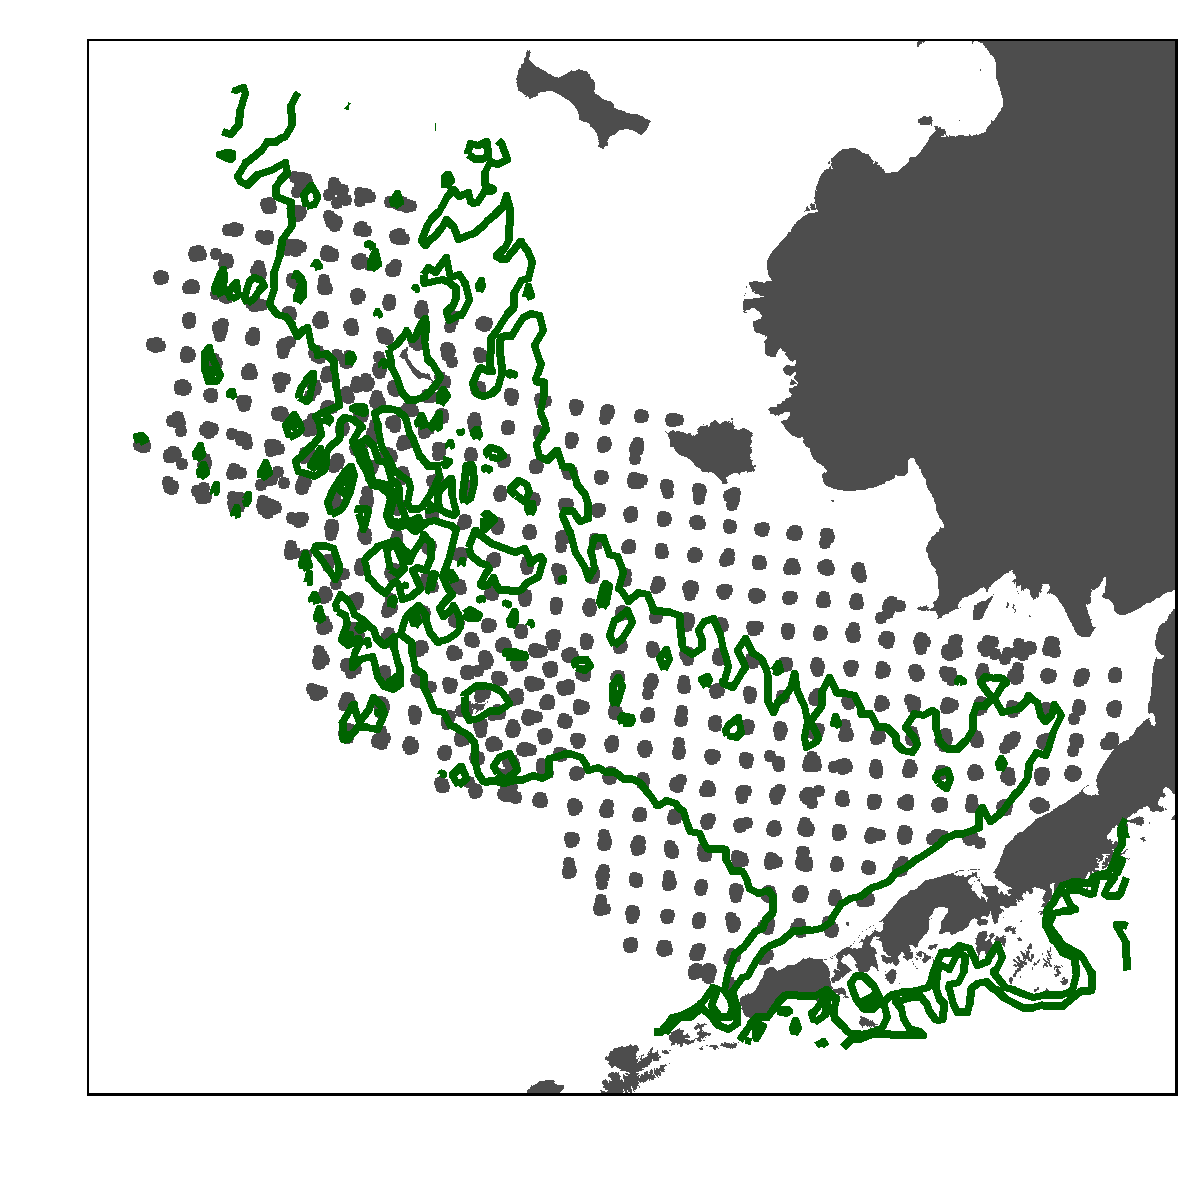
\includegraphics[width=16.67in]{C:/Users/Owen.Liu/Documents/github/cod_vs_crab/manuscript/figures/bathy_samples} \caption{The study area in the eastern Bering Sea. Locations of trawl survey data points used to train the spatial dynamic factor analysis model are shown in gray. Green bathymetric lines indicate the 50 and 100m depth contours, which broadly delineate the coastal, middle, and outer domains of the Bering Sea referred to in the text.}\label{fig:bathy}
\end{figure}

\hypertarget{data-and-methods}{%
\section{Data and Methods}\label{data-and-methods}}

\hypertarget{trawl-survey-data}{%
\subsection{Trawl survey data}\label{trawl-survey-data}}

To investigate the spatial patterns in Pacific cod and snow crab distributions as they vary over time, we use a joint dynamic species distribution model(JDSDM)\textsuperscript{24}. JDSDMs estimate ``factors'' representing latent spatial and spatio-temporal patterns in observed data. We fit the model to fishery-independent bottom trawl survey data from the Gulf of Alaska. The survey, conducted each summer, enumerates all species caught in each of approximately 375 tows across a 20 by 20 nautical mile grid, providing an annual census of the Bering Sea demersal fish and invertebrate communities (full survey details can be found at \url{https://www.fisheries.noaa.gov/resource/document/groundfish-bottom-trawl-survey-protocols}). Along with the number and weight of species caught, the survey also records near-bottom temperature, depth, and area swept by the trawl. For both cod and crab, all individuals are sexed and measured by fork length (FL) for cod or carapace width (CW) for crabs. Additionally, the survey denotes crab maturity stage, enabling us to distinguish between immature and mature crabs.

From the survey data, we extract all observations of snow crab and cod, then sort them into size bins. For snow crab, we defined two classes: immature and mature females. We defined immature crabs as crabs of both sexes that were smaller than 58 mm CW and sexually immature. The 58 mm cutoff is based on a diet study that found that 95\% of all crabs found in Pacific cod stomachs are smaller than 58mm. We define mature female crabs as any mature females, regardless of egg-carrying status or size. Size at maturity for snow crabs varies with latitude and year, although in most regions and years, primipara (first-time female spawners) are larger than 50 mm CW\textsuperscript{19}.

For Pacific cod, we enumerate total abundance at each survey station for cod within three size classes. As with snow crab, our size classes were based on previous studies of cod predation, which found that cod containing snow crabs in their stomachs were bewtween 200 and 800 mm FL\textsuperscript{20,21}. We define small cod as those \textless{}200 mm FL, medium cod as between 200 and 800 mm, and large cod as larger than 800 mm. Therefore, with our definitions, we would expect a predation interaction between medium cod and immature snow crab. Size frequency distributions for all classes used in the model are shown in the Supplementary Materials. In the following, we refer to the two crab and three cod categories in the data as ``classes''.

Temperature and depth are included as environmental covariates in the model described below. To ensure the environmental covariates matched the observed data as closely as possible, we extracted near-bottom temperature and depth directly from the survey itself, and then used inverse-distance weighting to interpolate values between survey points.

\hypertarget{joint-dynamic-species-distribution-model}{%
\subsection{Joint dynamic species distribution model}\label{joint-dynamic-species-distribution-model}}

We implement the JDSDM through the publically available Vector Autoregressive Spatiotemporal R package \texttt{VAST}. VAST uses a delta-generalised linear mixed modeling method, and takes into account spatio-temporal correlations among species (or size classes of one species, as in our model). A full description of the modeling framework can be found elsewhere\textsuperscript{24,25}, but we describe the key equations here.

The JDSDM models response variables as a multivariate process where the predicted abundance of a class at a location is represented as the combination of two linear predictors: encounter rate (i.e., presence/absence of a class at a given location), and positive catch rate (i.e., the prediction of abundance given the presence of a class in a location). VAST estimates fixed and random effects for the two linear predictors that are each a function of an intercept, a spatial effect, a temporal effect, and any density covariates. In our model, bottom temperature and depth were used as density covariates. More specifically, the first linear predictor represents encounter rate for sample \(i\) as,

\begin{equation}
  p_1(i)=\beta_1(c_i,t_i)+\sum_{f=1}^{n_{\omega1}}L_{\omega1}(c_i,f)\omega_1(s_i,f)+\sum_{f=1}^{n_{\epsilon1}}L_{\epsilon}(c_i,f)\epsilon_1(s_i,f,t_i)+\sum_{p=1}^{n_p}\gamma_1(c_i,t_i,p)X(s_i,t_i,p)
  \label{eq:linpred}
\end{equation}

where \(p_i\) is the linear predictor for encounter rate, \(\beta_1(c_i,t_i)\) is the intercept term in year \(t\) for class \(c\), the terms starting with \(L_\omega\) and \(L_\epsilon\) are the spatial and spatio-temporal factor models, respectively, and \(X\) is the matrix of density covariates defined for each location \(s\), time \(t\) and covariate \(p\) that have linear effects \(\gamma\) on the predictor. In the factor model terms, \(L\omega\) and \(L_\epsilon\) are loading matrices relating the classes to each of \(f\) factors, and \(\omega(s,f)\) and \(\epsilon(s,f,t)\) are vectors of random effects representing latent spatial and spatio-temporal variation at each location. VAST models average spatial variation \(\omega\) as being constant across years, while spatio-temporal variation \(\epsilon\) varies among years. The second linear predictor, representing positive abundance, has an analogous formulation.

We use a log-link to transform both linear predictors to predict the observed data (see Thorson 2019 for all model equations):

\begin{equation}
  r_1(i) = 1-exp(-a_i\times exp(p_1(i)))
  r_2(i) = \frac{a_i\times exp(p_1(i))}{r_1(i)\times exp(p_2(i))}
  \label{eq:transpred}
\end{equation}

where \(a_i\) is the area associated with sample \(i\) in the survey. Positive abundance is modeled with a gamma distribution.

An important feature of VAST is that it accounts for spatial autocorrelation, or that fact that values nearby in space tend to be more similar than locations further away. Each spatial (\(\omega\)) and spatio-temporal (\(\epsilon\)) factor in both linear predictors are represented as Gaussian random fields, where the covariance between nearby locations is approximated with a Matern correlation function\textsuperscript{26} through the R-INLA software\textsuperscript{27}. The correlation function follows geometric anisotropy, where the rate of decline in correlation between locations decline can be different in different directions (i.e., correlation can decline more rapidly in the east-west than the north-south direction).

Parameter estimation for VAST is accomplished through Laplace approximation of the marginal likelihood for fixed effects while integrating across the random effects using the Template Model Builder software\textsuperscript{28}. The model requires the estimation of 87 fixed effects and 25752 random effects. For this study, we are primarily interested in the spatial and spatio-temporal factors, and how the five classes in our study relate to those factors, represented by the factor loadings matrices. We estimated three spatial and three spatio-temporal factors for both linear predictors, while including temperature and depth as covariates. As derived quantities, VAST can also calculate each class' spatial abundance-weighted center of gravity and effective area occupied within the EBS, as well as an overall (non-spatial) index of abundance. We use these derived quantities to further explore the spatial and temporal dynamics of snow crab and cod.

\hypertarget{results}{%
\section{Results}\label{results}}

\hypertarget{dominant-spatial-and-spatio-temporal-patterns}{%
\subsection{Dominant spatial and spatio-temporal patterns}\label{dominant-spatial-and-spatio-temporal-patterns}}

We estimate three factors for spatial and spatio-temporal variation in the five classes (two snow crab and three Pacific cod classes). To visualize the factors, we estimate all spatial values within 100 distinct spatial regions across the EBS, analytically chosen to minimize the average distance between those locations and the available data. Immediately, there are clear, interpretable patterns apparent in the average spatial variation of cod and crab. These patterns manifest in both the northeast-to-southwest dimension (the longer axis), and the cross-shelf or shorter axis of the EBS. Figure \ref{fig:omegas} shows the spatial distribution of the first two factors describing presence/absence and positive abundance. These maps show the most important spatial patterns in cod and crab distribution across the EBS. The first factors for both encounter rate and positive abundance (panels a and c of Figure \ref{fig:omegas}) have positive values in the southeast towards Bristol Bay, increasing to positive values with greater depth and latitude. The second factors for encounter rate and positive abundance show slightly different patterns. For encounter rate, positive values clearly delineate the mid-depth band of the EBS. It is strongly and significantly associated with lower temperatures (Pearson's \(\rho\) -0.51), picking up the signal of the EBS cold pool. The second factor for positive abundance shows a transverse pattern across the shelf from northeast to southwest, and is also significantly associated with temperature (\(\rho\) 0.47).

\begin{figure}
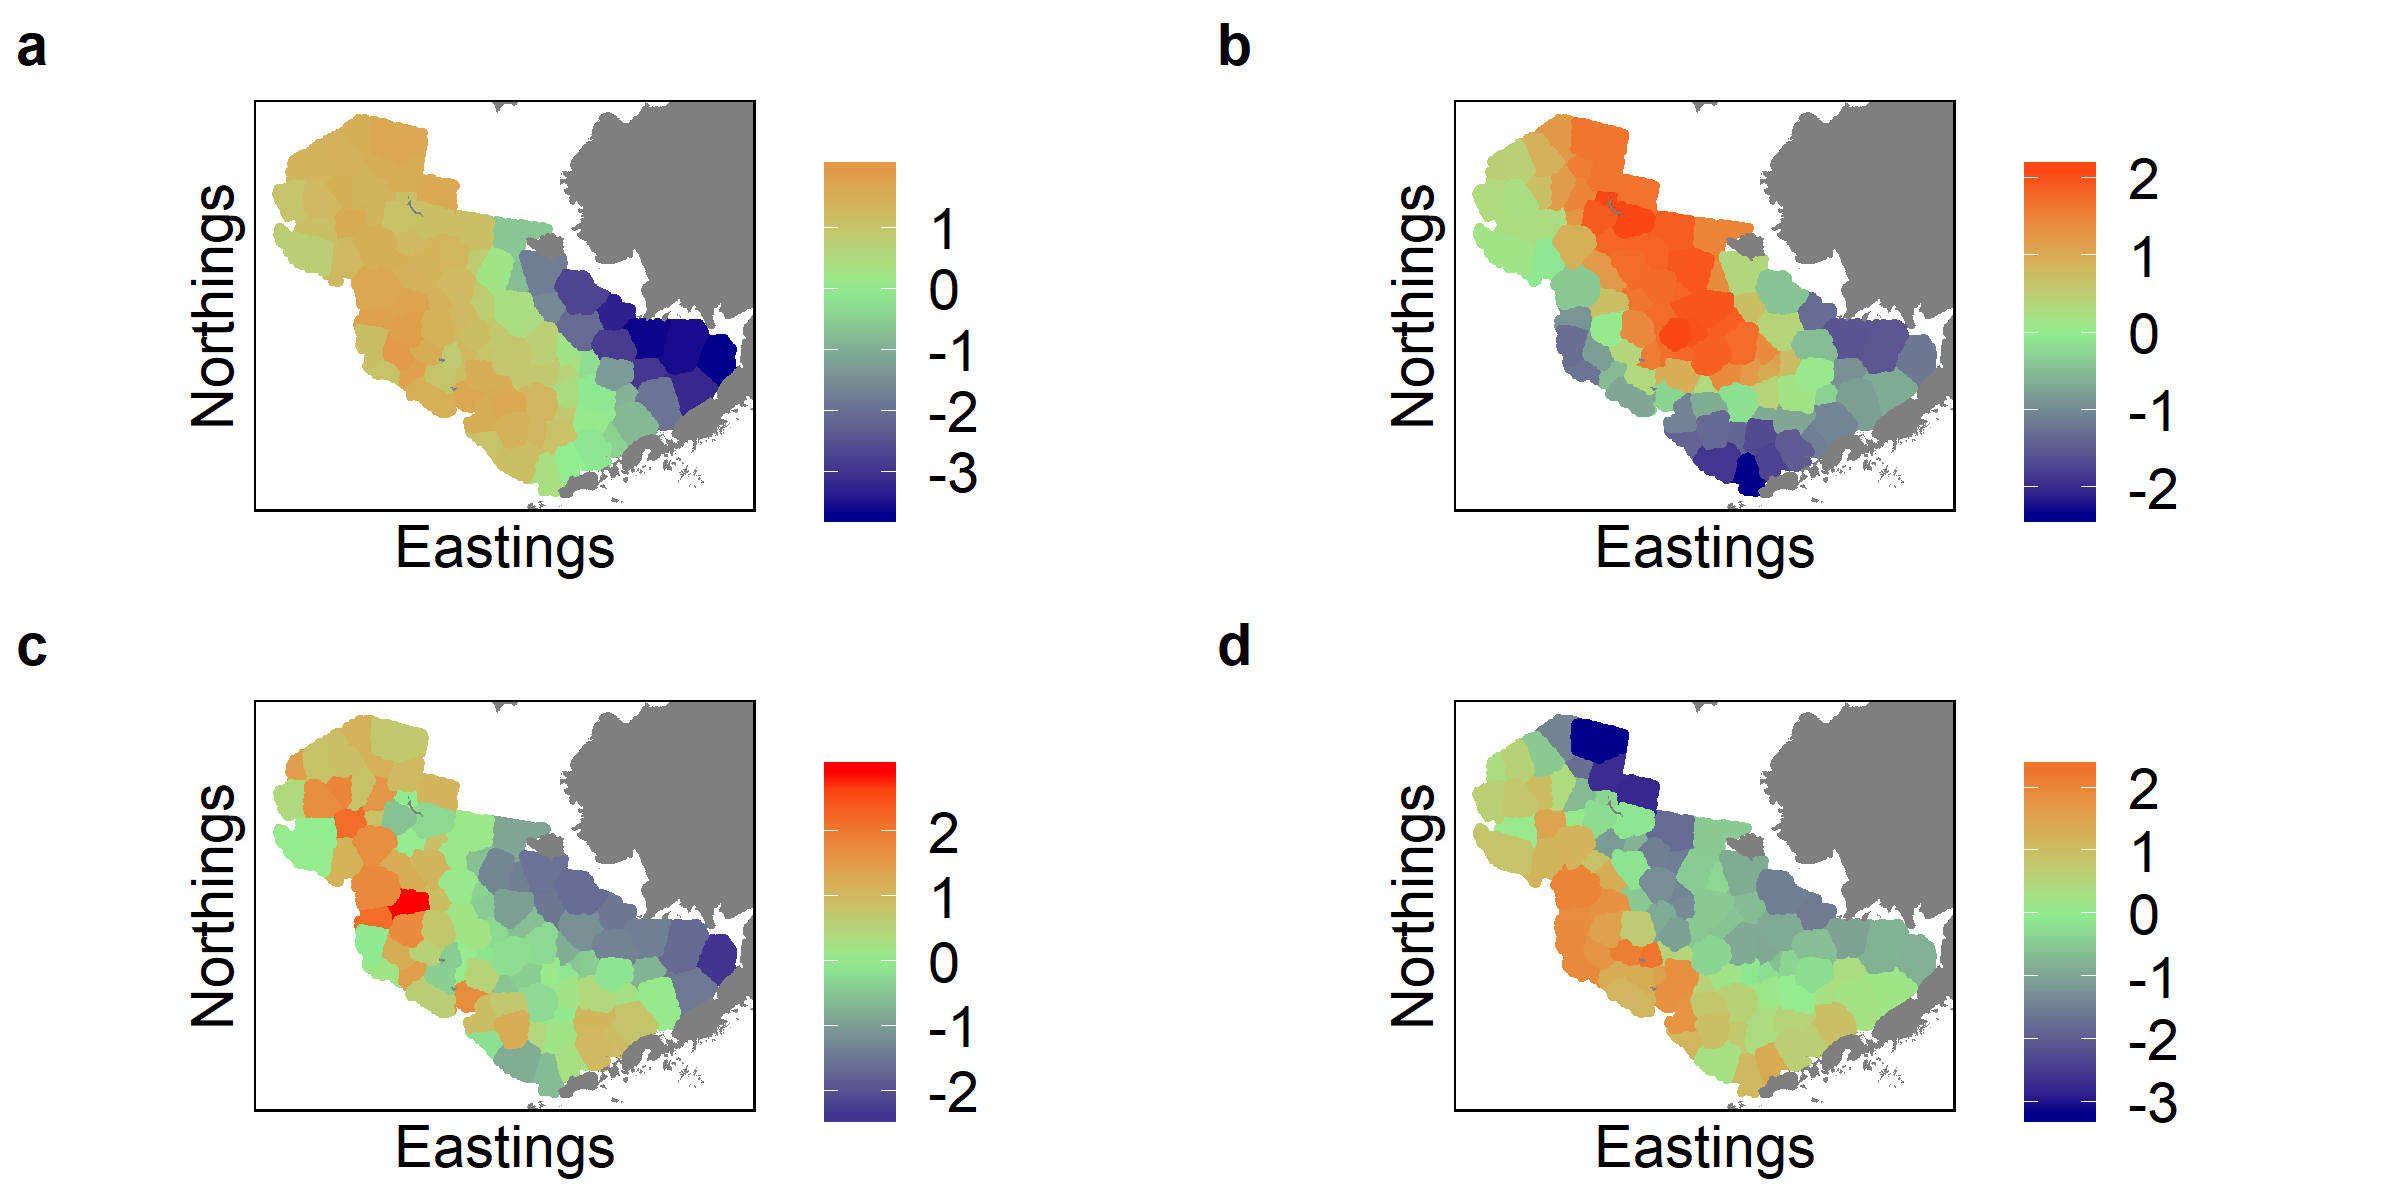
\includegraphics[width=33.33in]{C:/Users/Owen.Liu/Documents/github/cod_vs_crab/manuscript/figures/omegas} \caption{The first two spatial factors describing encounter rate (presence or absence,panels a and b) and positive abundance (panels c and d) of snow crab and Pacific cod in the EBS. Panels a and c are the first factor of encounter rate and positive abundance, respectively, and panels b and d are the second factors. Warmer colors represent positive values of the factor, while cool colors represent negative values.}\label{fig:omegas}
\end{figure}

Figure \ref{fig:omegas} shows the main static patterns in size-structured cod and crab distributions in the EBS, but we can also investigate the major patterns in species distributions over time through the estimation of spatio-temporal factors, i.e.~the \(\epsilon(s,f,t)\) terms in equation \eqref{eq:linpred}. These latent spatio-temporal factors are important in describing interannual variation in species distributions, but display complex temporal patterns. For example, consider Figure \ref{fig:epsilon} that shows the values of the first spatio-temporal factor for positive abundance (i.e., abundance given the presence of a class at a location). In many years, much of the factor is near zero, with occasional strong spatial signals in specific areas of the EBS. For example, in 1984 and 2015, the factor displays strong negative values in the Bristol Bay and southeastern coastal areas, while in 1993 to 1994 there are strong positive values in the northern coastal portion of the study area. Interestingly, the factor also shows negative values across the central and southwestern portions of the shelf from the mid-1990s to the mid-2000s, which is the period of documented distributional change in snow crab distribution\textsuperscript{13}.

The variation apparent in Figure \ref{fig:epsilon} is not clearly associated with near-bottom temperature anomalies across the study period. The average spatial values of the factor in each location across years are not signficantly correlated with average temperature anomaly (\(p\)\textgreater{}0.05), and while in certain years the relatoinship between the factor and temperature is significant, some of these correlations are positive and others are negative. It is likely, therefore, that the spatio-temporal factors represent the combined influence of a number of temporally-varying environmental and predation processes and are therefore difficult to interpret through any single environmental variable. Maps of all three factors for all four linear predictors are shown in the Supplementary Material.

\begin{figure}
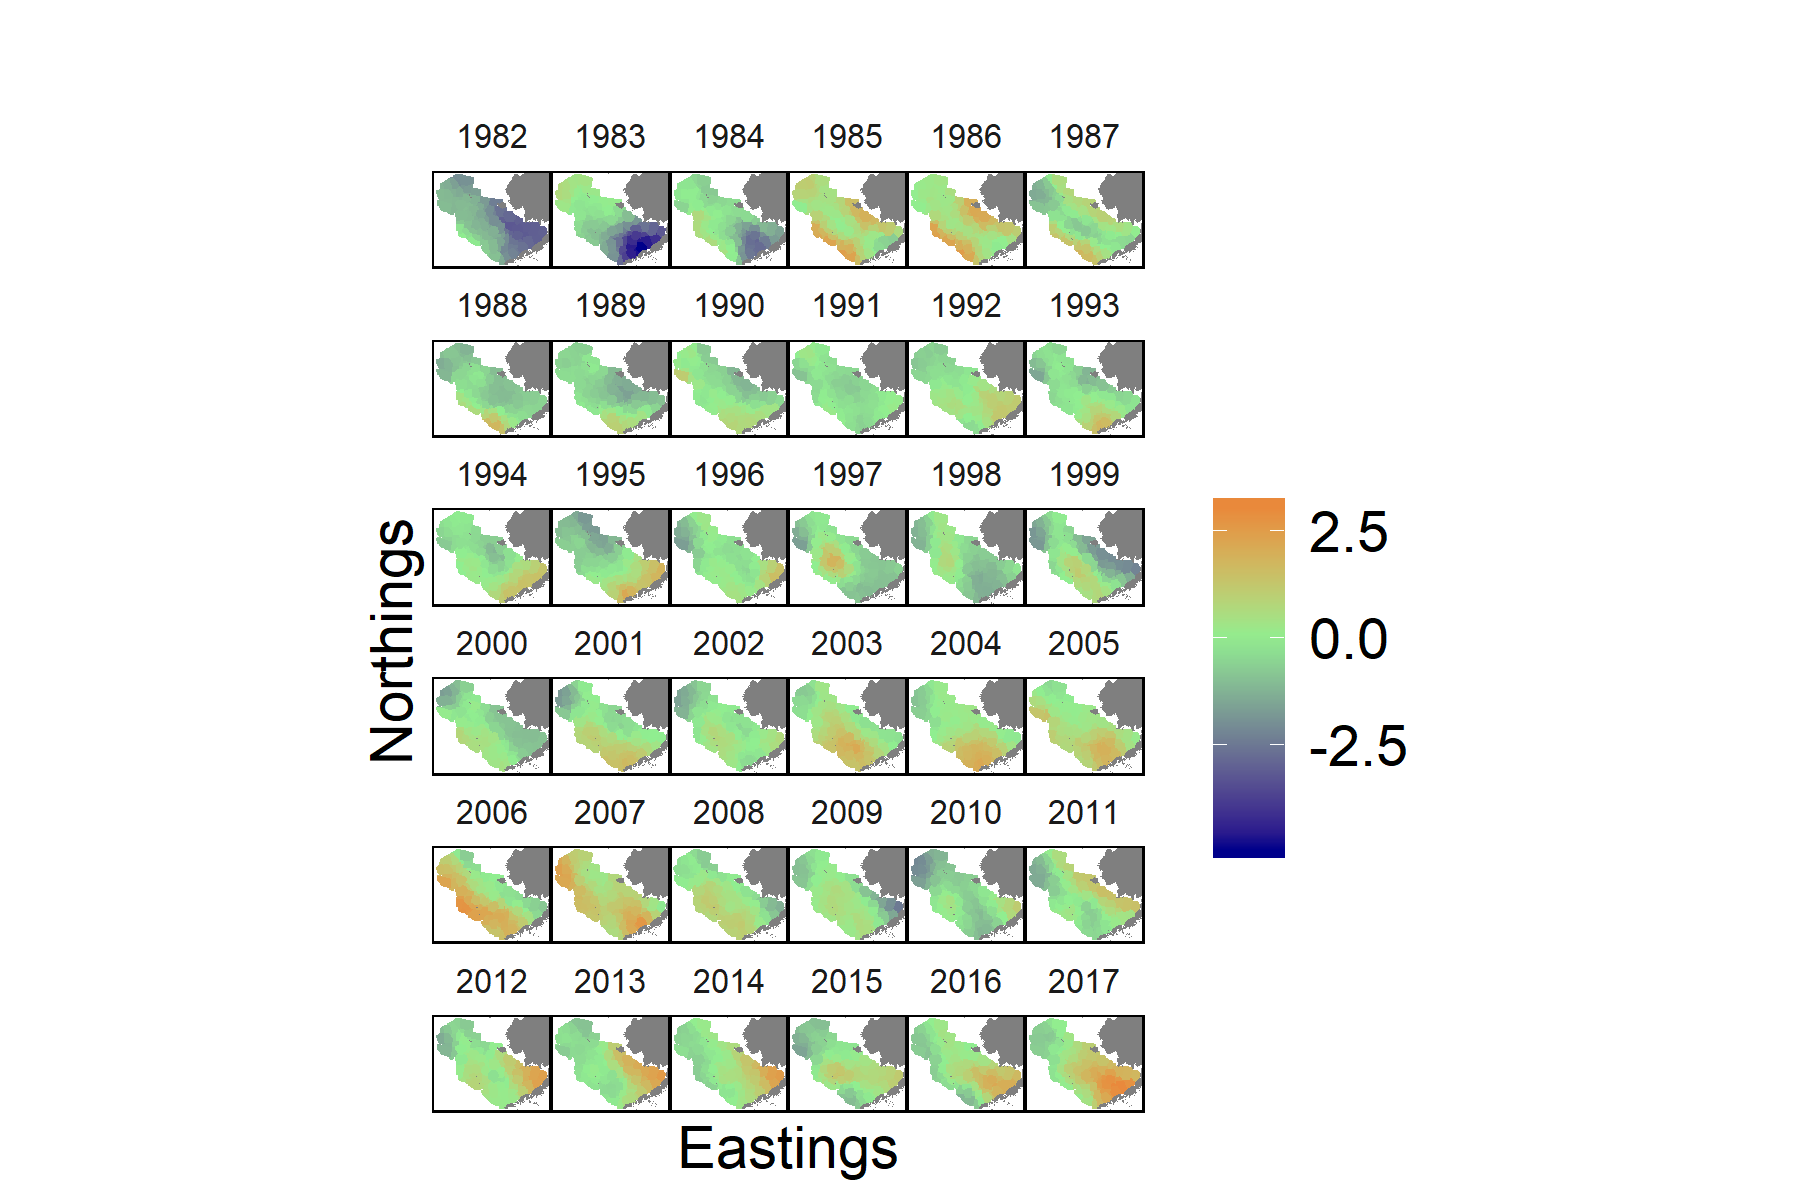
\includegraphics[width=25in]{C:/Users/Owen.Liu/Documents/github/cod_vs_crab/manuscript/figures/epsilon1} \caption{Values of the first spatio-temporal factor for encounter probability in each year in the study. Warmer colors represent positive values of the factor, while cooler colors represent negative values.}\label{fig:epsilon}
\end{figure}

\hypertarget{species-associations-with-spatial-and-spatio-temporal-factors}{%
\subsection{Species associations with spatial and spatio-temporal factors}\label{species-associations-with-spatial-and-spatio-temporal-factors}}

Figures \ref{fig:omegas} and \ref{fig:epsilon} show some of the major patterns in cod and crab distributions across the EBS, but to explore how each species associates with these patterns, we investigate the factor loading matrices \(L_\omega\) and \(L_\epsilon\). Figure \ref{fig:loads} shows the loadings of each species on to the three factors for each linear predictor. The first two factors for average spatial variation explain 85.1\% and 88.2\%, respectively of the between-class variance in encounter rates and positive abundance (the left two columns of Figure \ref{fig:loads}). Snow crab and cod show opposite relationships to the first spatial factor for both encounter rate and positive abundance. Snow crab, and mature females in particular, are strongly positively associated with the first factor, while small cod are negatively associated and medium and large cod have smaller loadings. The encounter probabilities of snow crab and small cod are positively associated with the second factor for average spatial variation in encounter probability, while all classes except immature crabs are positively associated with the second factor for variation in positive abundance.

The right two columns of Figure \ref{fig:loads} show how the presence and abundance of each class is related to annually-varying factors. Together, the first and second factors describing spatio-temporal variation in encounter rates explained 84.8\% of between-species variance. The first factor shows clear differences between species, where snow crabs are negatively associated and Pacific cod positively associated. conversely, crab and large cod are positively associated with the second factor, while small cod is negatively associated. Finally, the first factor describing spatio-temporal variation in positive abundance primarily represents the distributions of the two crab classes. The second factor for spatio-temporal variation in positive abundance separates the two crab classes, where the positive abundance of immature crabs is negatively associated and the abundance of spawners positively associated. The third factor in all four linear predictors show more positive associations across all classes, but explains a much smaller proportion of overall variance in cod and crab distributions. However, the third factor seems to be where much of the variance in the distribution of medium-sized cod is contained---the highest loading of medium cod on to any factor is for the third factor of spatio-temporal variation in positive abundance.

\begin{figure}
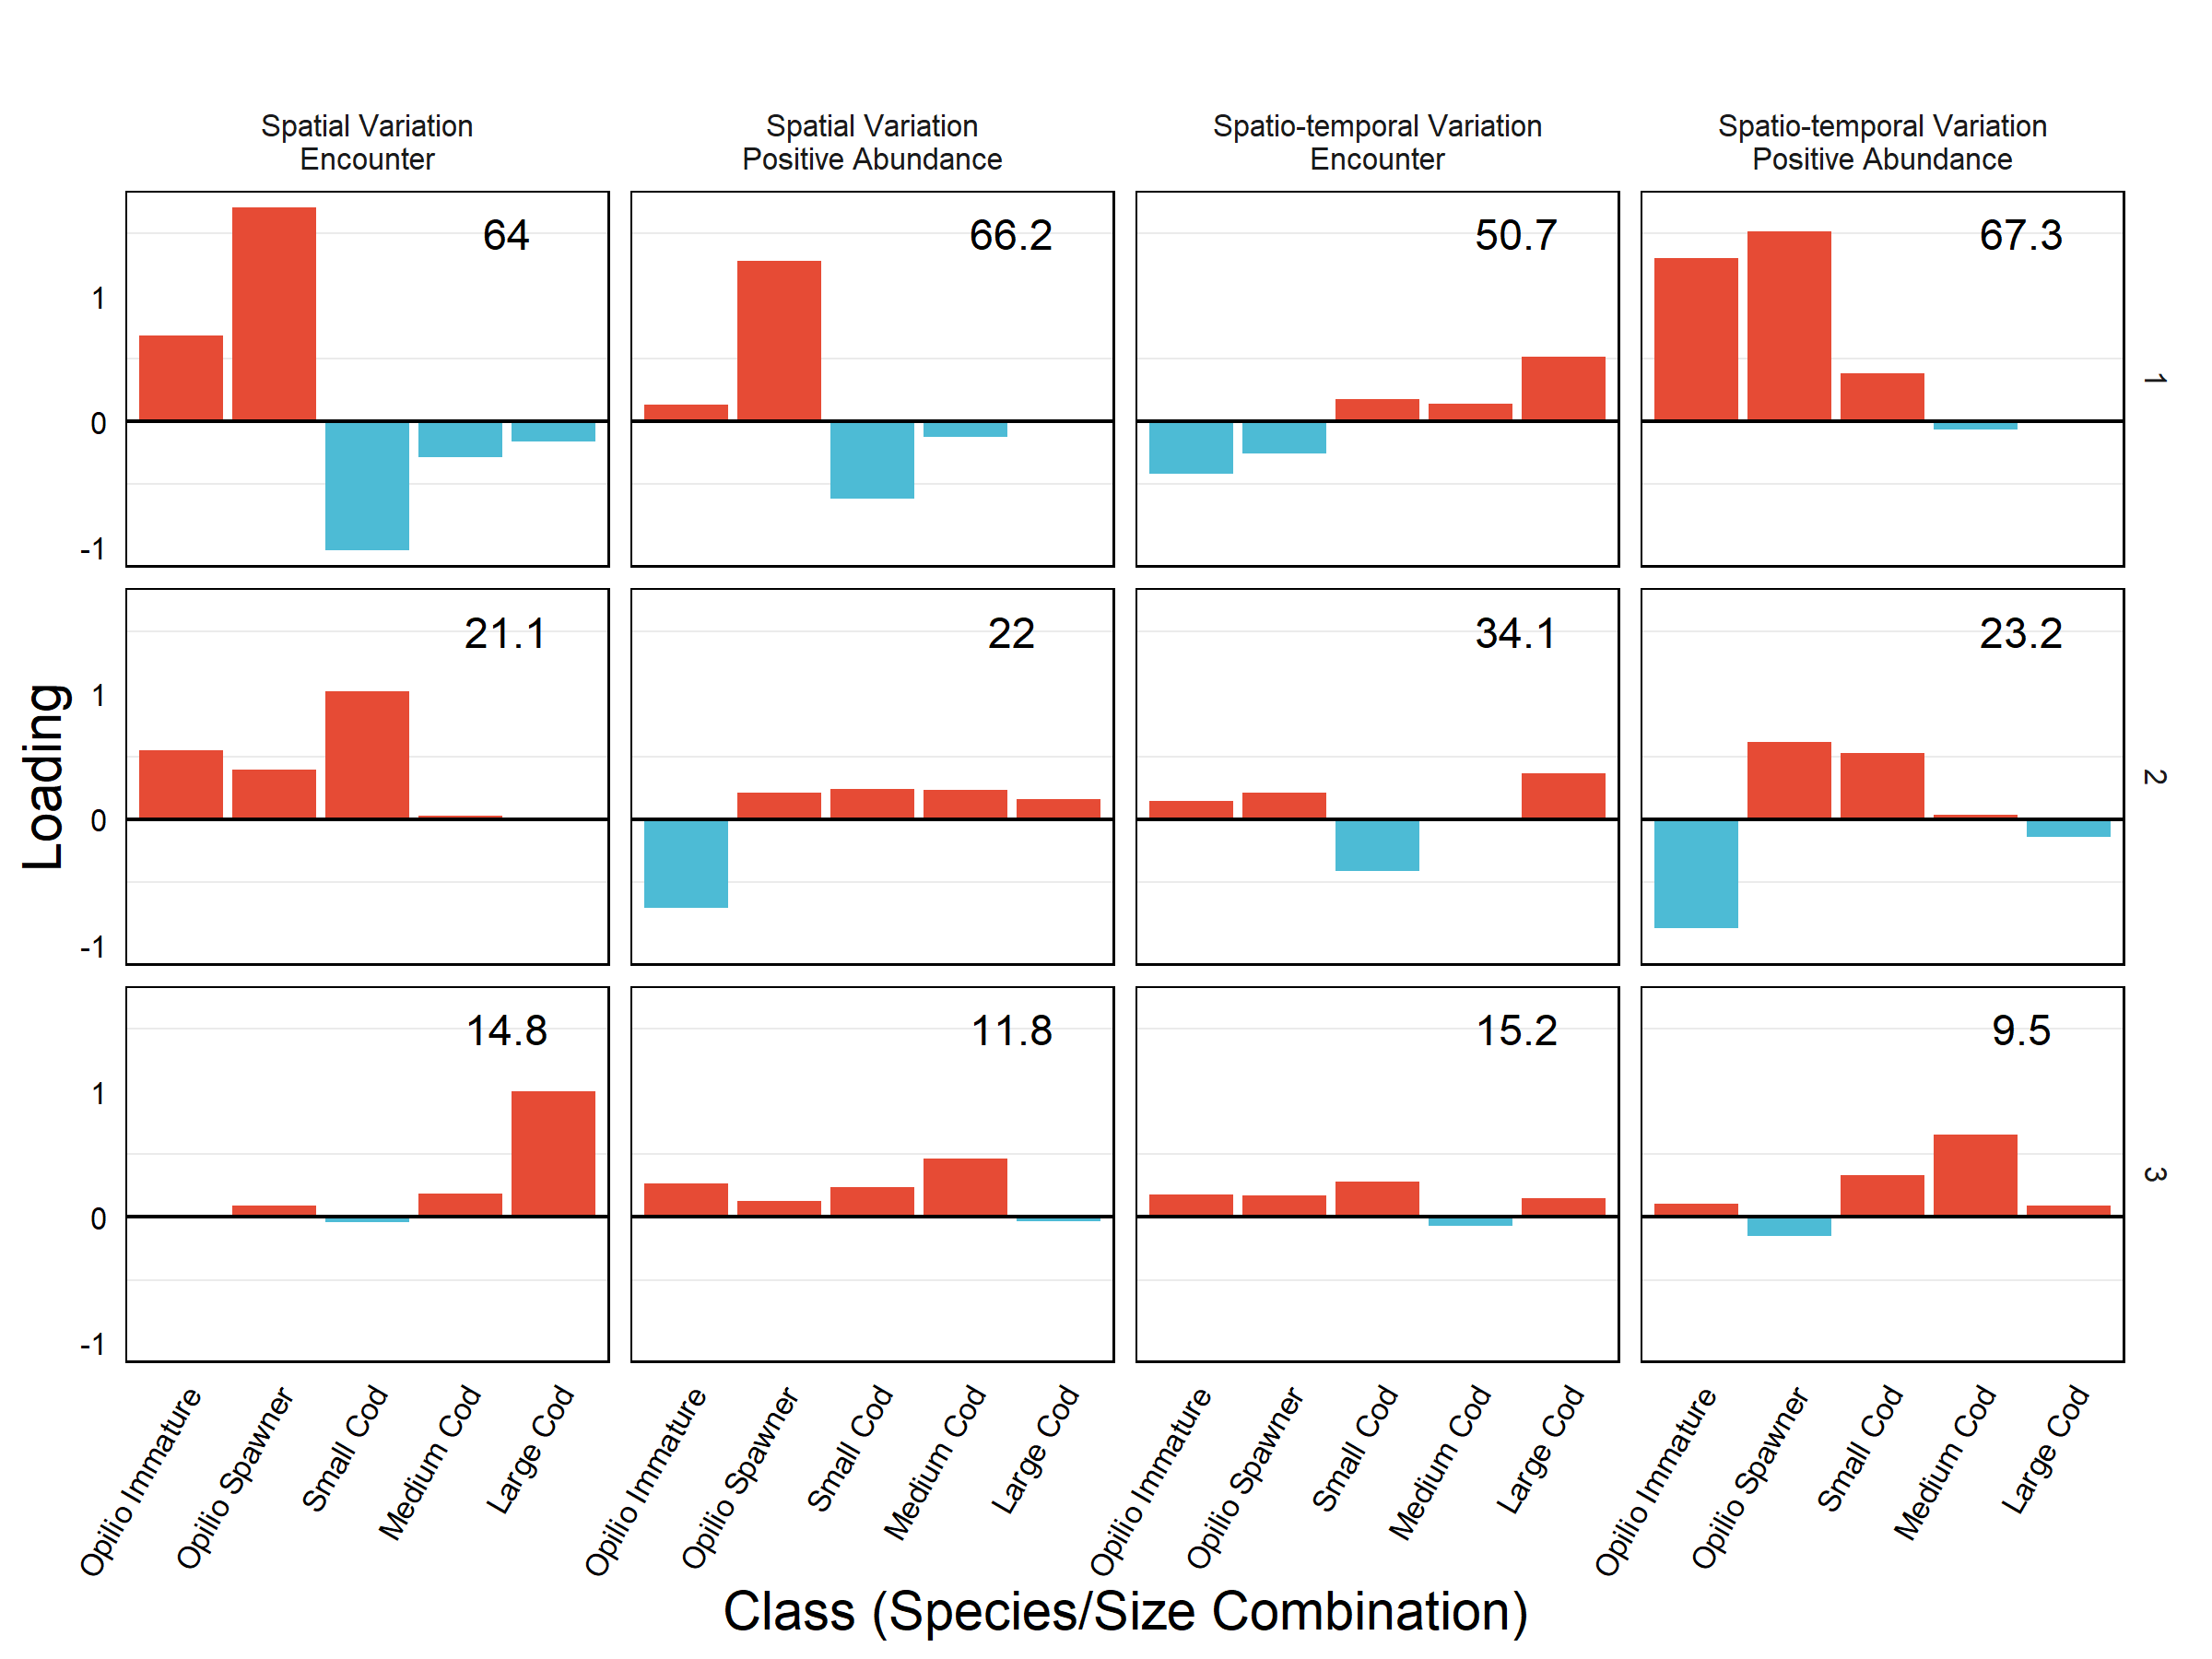
\includegraphics[width=33.33in]{C:/Users/Owen.Liu/Documents/github/cod_vs_crab/manuscript/figures/fct_loadings} \caption{Factor loadings for each class (bars), linear predictor (columns) and factor (rows), where positive loadings are shown in red and negative loadings in blue. Numbers in the upper right corner indicate the overall between-class variance explained by each factor. The five classes are small immature snow crab (Opilio Immature), spawner snow crab (Opilio Spawner), and small (<200mm FL), medium (between 200 and 400mm), and large (>800mm) Pacific cod.}\label{fig:loads}
\end{figure}

Figure \ref{fig:loads} suggests that for the most, crab and cod respond in divergent ways to the spatial and spatio-temporal patterns described above. The separation between species is more clearly evident when plotted in two-dimensional space. For instance, Figure \ref{fig:2dfcts} shows the first two factors describing spatio-temporal variation in the positive abundance of all five classes in the study. Clearly, the two species are distinguished along the first factor, while the second factor segregates immature from mature crabs. Medium and large cod have little relationship to either factor, but small cod is associated positively with both factors.

\begin{figure}
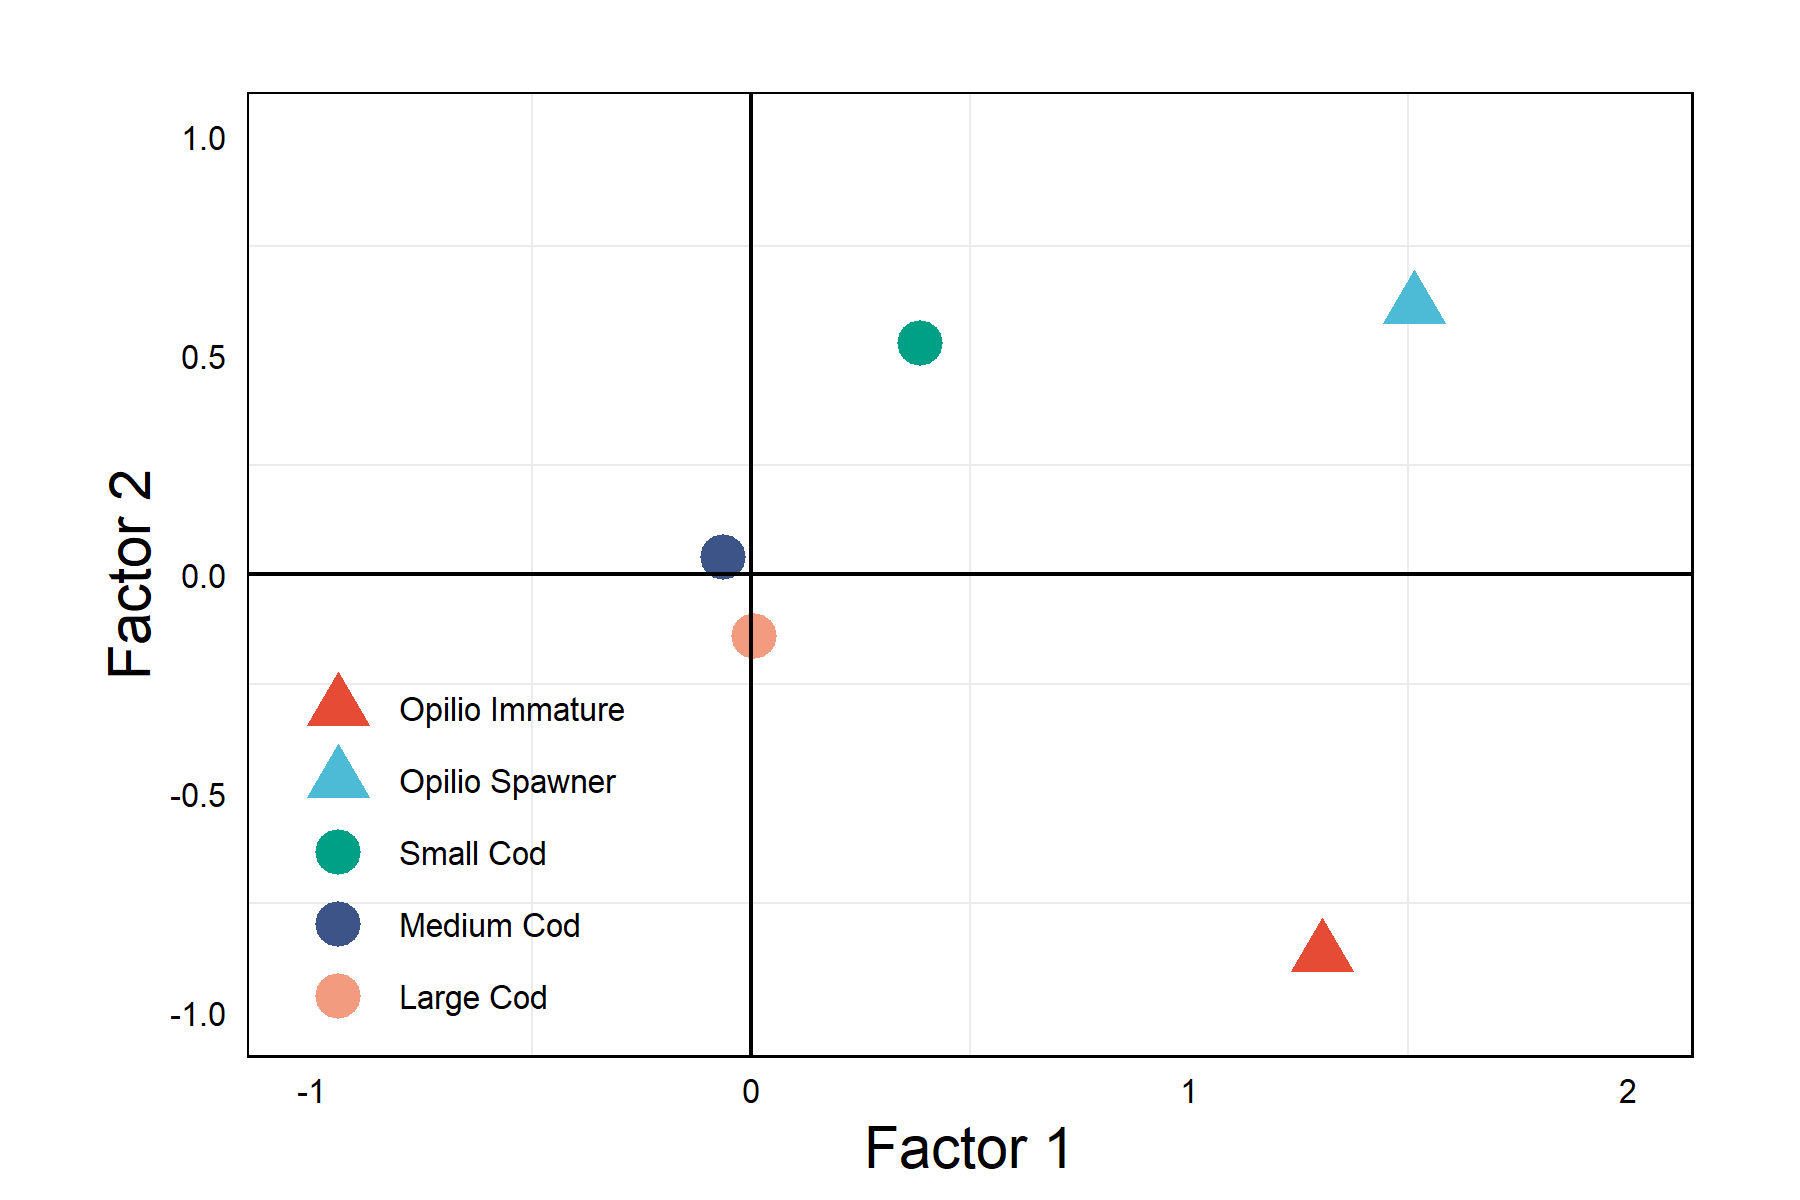
\includegraphics[width=25in]{C:/Users/Owen.Liu/Documents/github/cod_vs_crab/manuscript/figures/epsilon22d_fcts} \caption{Loadings of all classes on to the first two factors for spatio-temporal variation in positive abudance. Triangles indicate snow crab classes and circles indicate cod classes.}\label{fig:2dfcts}
\end{figure}

Comparing factor loadings (Figures \ref{fig:loads} and \ref{fig:2dfcts}) to factor maps (Figures \ref{fig:omegas} and \ref{fig:epsilon}) gives a view of the major patterns in each species' distribution. For example, the average encounter probability for immature snow crab is described well by the first factor (panel (a) in Figure \ref{fig:omegas}), showing that on average, immature crabs are more likely to be found towards the northern section of the EBS, and much less likely to occur in the Bristol Bay region. At the same time, we know from Figures \ref{fig:loads} and \ref{fig:2dfcts} that distributional change over time in the same class is well-described by the first spatio-temporal factor for positive abundance. The map of this factor (Figure \ref{fig:epsilon}) clearly represents the major distributional changes in the snow crab stock over time.

\hypertarget{species-center-of-gravity}{%
\subsection{Species center-of-gravity}\label{species-center-of-gravity}}

Together, the factors describing the variations in distribution of cod and crab across the EBS result in predictions of their abundances across space. Predicted total abundance in any location is simply the product of encounter rate and positive abundance and is produced as a derived quantity in our analysis. Along the same lines, we can derive measures of the abundance-weighted center of gravity of each class to explore how that center has varied over time, as well as an overall non-spatial index of stock abundance. Although we can map species distributions across space and time (see predicted abundance plot for immature snow crab in the Supplementary Materials), the important general trends in species distributions are apparent in their centers-of-gravity. In Figure \ref{fig:cog}, it is clear that in general, the bulk of snow crab abundance is centered towards the north and west, while small cod occur in the south and east (Bristol Bay). The center of larger-sized abundances of both species occur towards further to the south and west than their smaller counterparts, more towards the middle and outer portions of the EBS shelf.

\begin{figure}
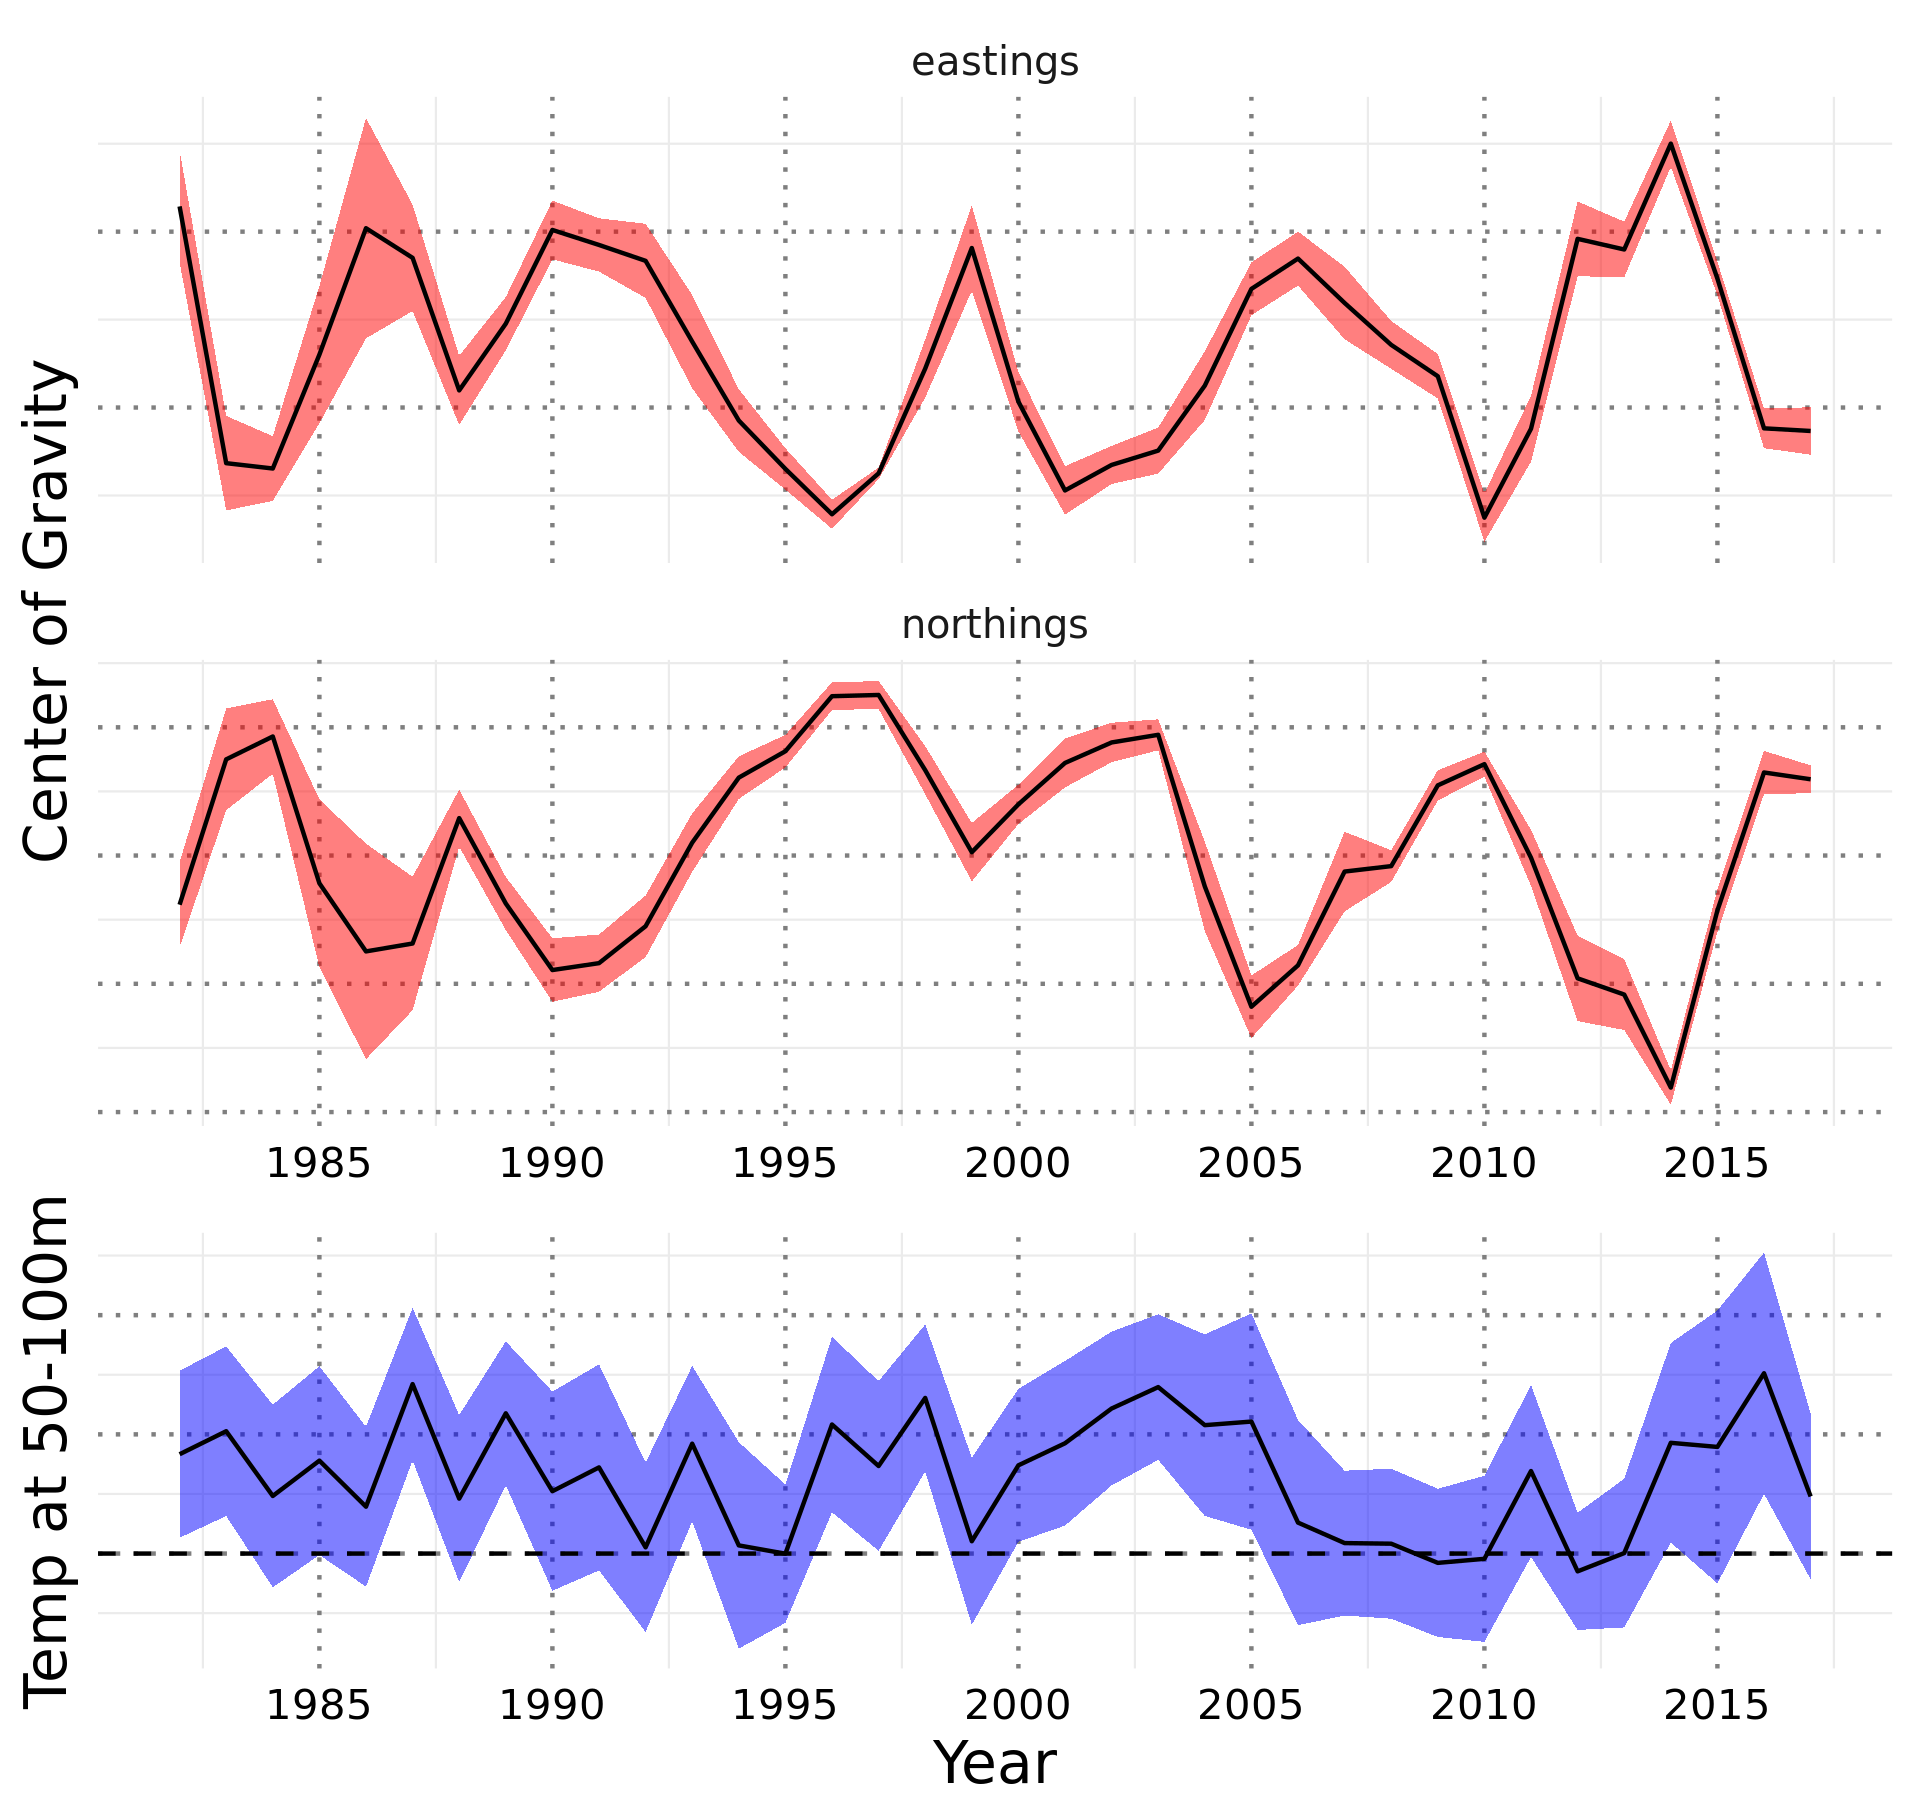
\includegraphics[width=33.33in]{C:/Users/Owen.Liu/Documents/github/cod_vs_crab/manuscript/figures/cog} \caption{Eastward (top row) and northward (bottom row) components of abundance-weighted center of gravity for each class (columns) across the study period.}\label{fig:cog}
\end{figure}

There have also been major changes in these species and size-specific centers of gravity over time. In particular, the north-south fluctuations in the snow crab distribution are clearly evident, with a rapid northward shift in the juvenile distribution of approximately 150 km from the mid-1990s to the mid-2000s, corresponding to the period of severely depressed landings in the snow crab fishery. In more recent years, a strong shift in cod distribution is apparent, with the distribution of small cod retreating to the south and east over time. Since the mid-2000s, the distributions of medium and large cod have also shifted east and towards the inner or coastal domain of the EBS.

\hypertarget{relationships-between-abundance-and-temperature}{%
\subsection{Relationships between abundance and temperature}\label{relationships-between-abundance-and-temperature}}

Lastly, we can use the derived abundances of each class to explore significant relationships among species abundances and between species abundances and environmental variables. We find no strong correlations---positive or negative---between overall abundances of classes, when we combine data across all locations (Figure \ref{fig:corrs}a). This is contrary to our hypothesis that immature snow crab and medium-sized cod abundances should be negatively correlated (in fact, they show a significant positive, if small, correlation). However, when we separate correlation estimates across space, a clearer picture begins to emerge. Figure \ref{fig:corrs}b shows the correlation between medium cod and immature crab abundance, calculated across years but separately for each spatial location. Medium cod and immature crab abundance are strongly negatively correlated in Bristol Bay and in the coastal domain of the EBS (throughout much of the core distribution area of cod), but not significantly correlated in the rest of the study area except for small pockets in the middle and far northwest domains of the study area.

\begin{figure}
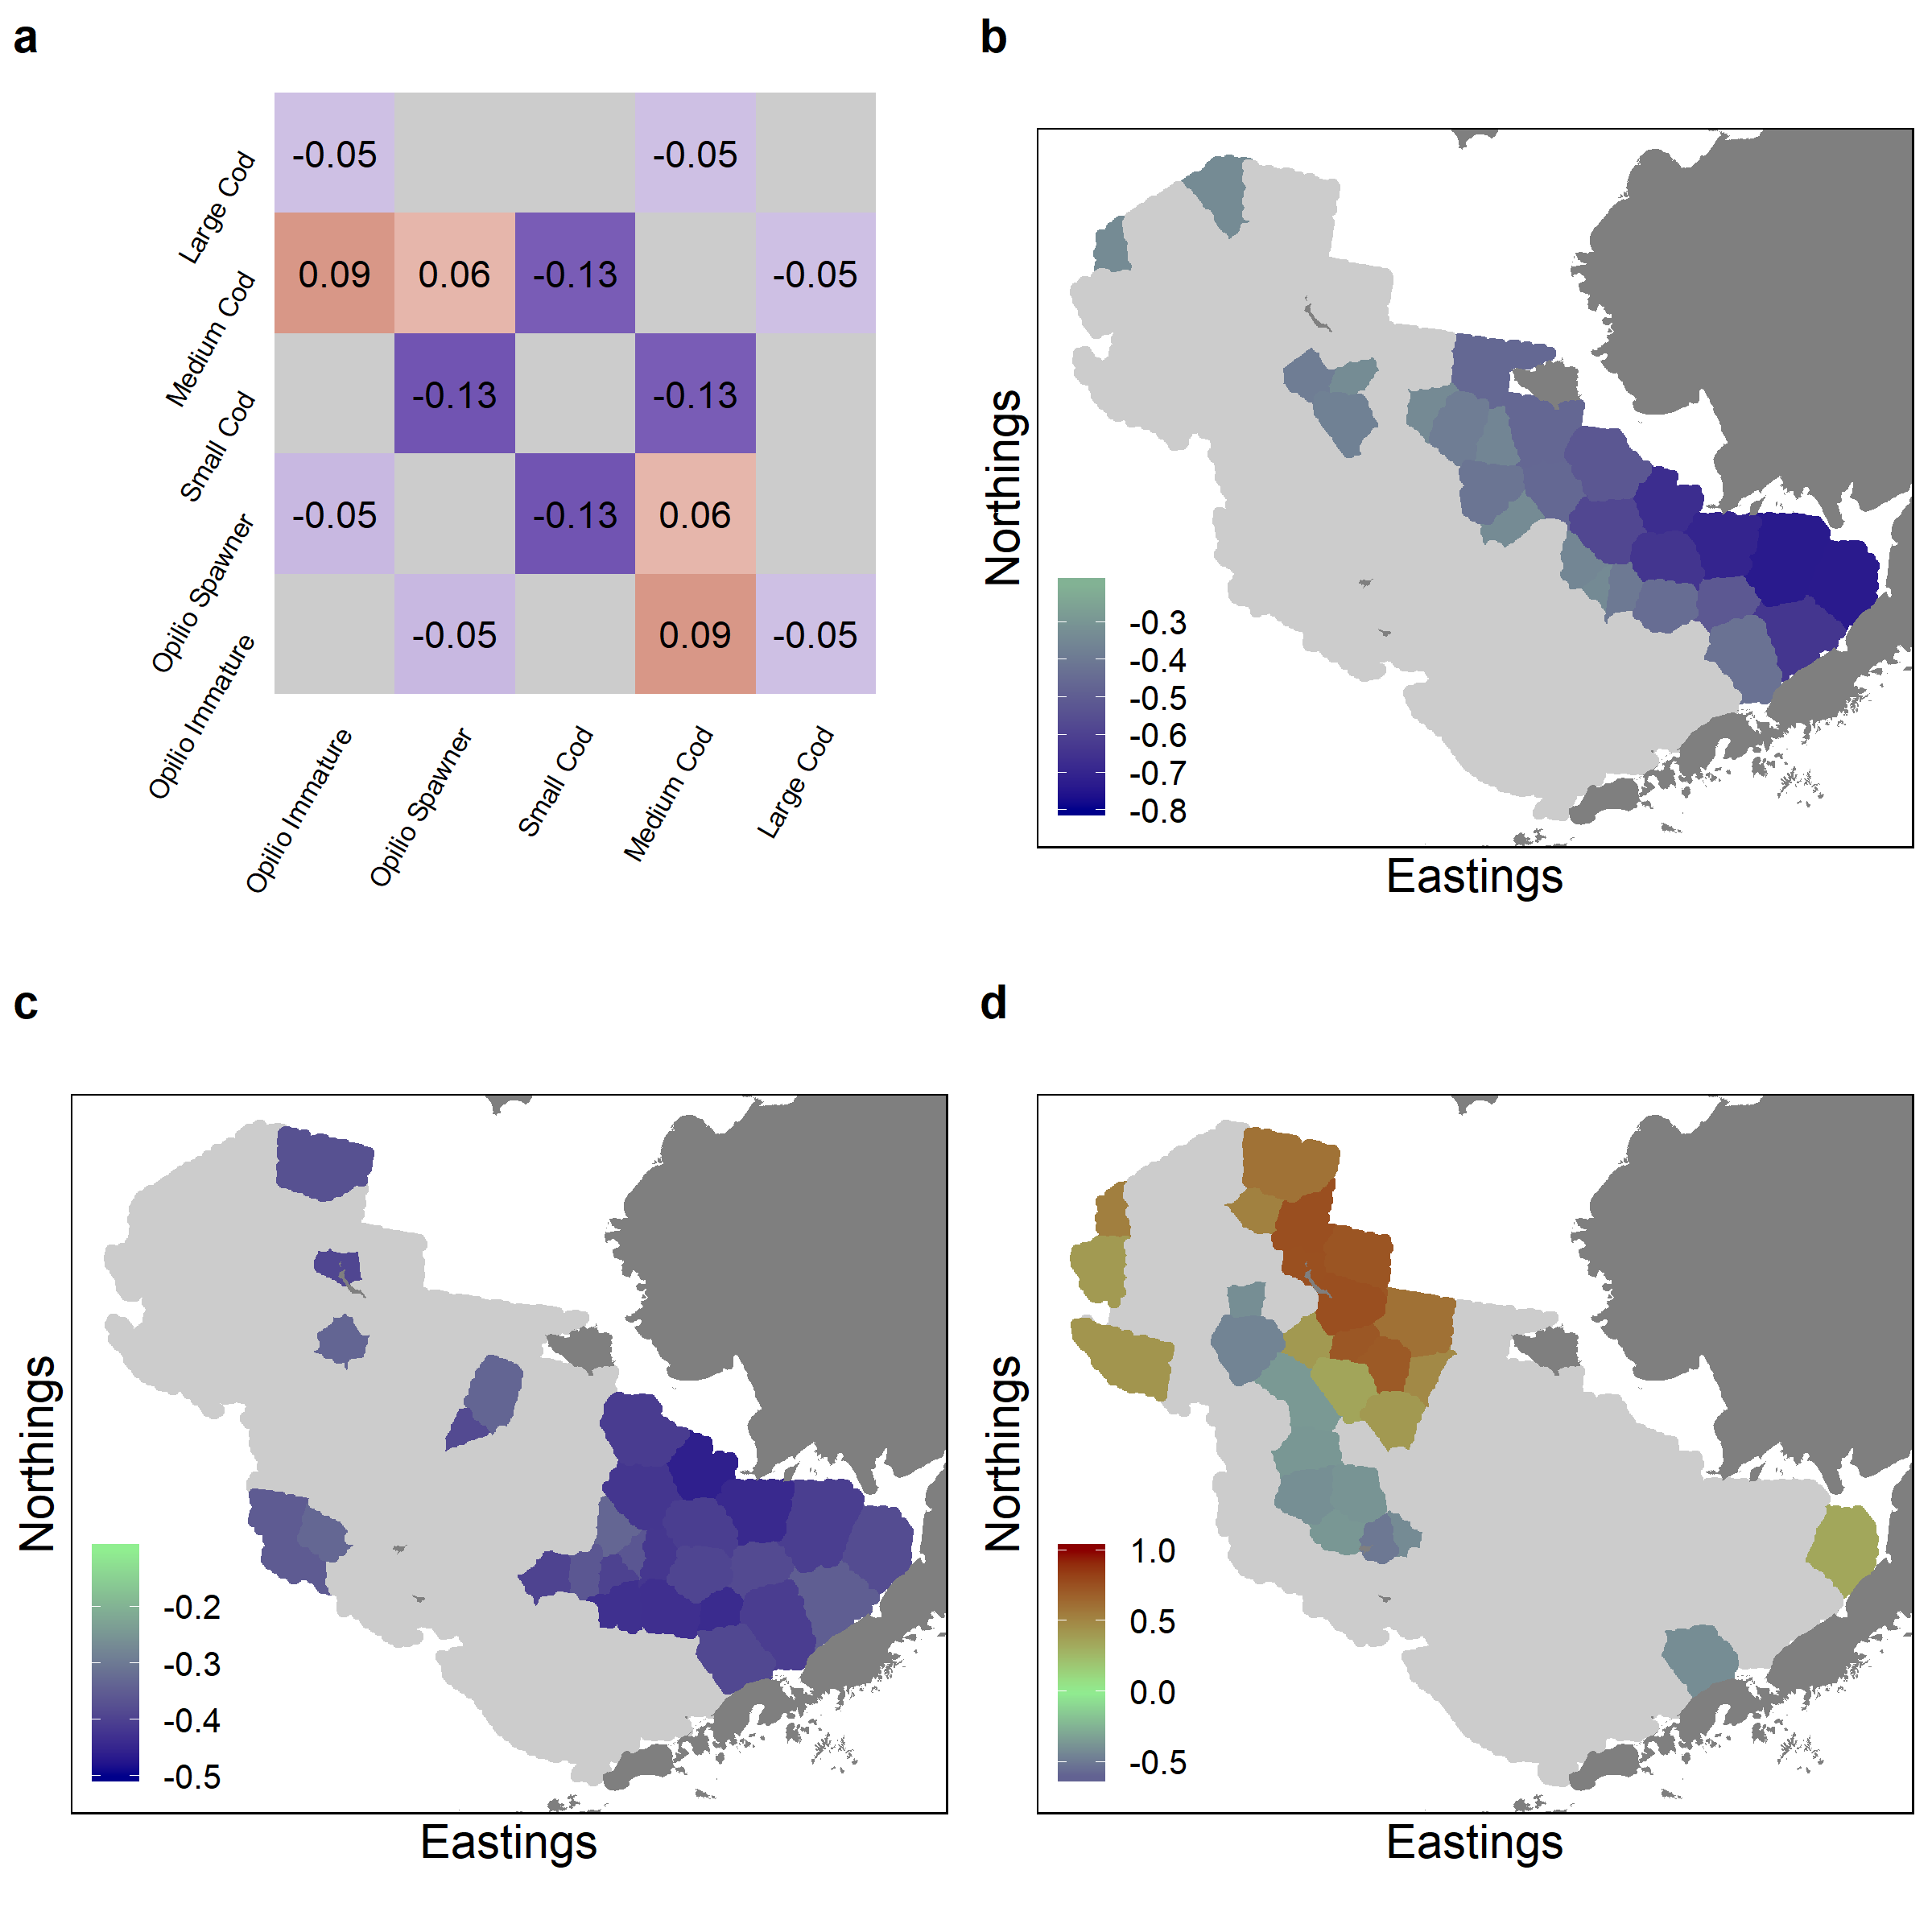
\includegraphics[width=33.33in]{C:/Users/Owen.Liu/Documents/github/cod_vs_crab/manuscript/figures/corrs} \caption{Correlations between species abundances and between abundances and temperature. In all panels, cool colors indicate negative correlations, while warm colors indicate positive correlations and gray indicates non-significant correlation. (a)Correlations in predicted abundances of all species across all locations. (b)Spatial correlations between predicted abundances of medium-sized cod and immature snow crab. (c)Spatial correlations between immature snow crab and annual near-bottom temperature anomalies. (d)Spatial correlations between medium-sized cod and annual near-bottom temperature anomalies.}\label{fig:corrs}
\end{figure}

The strong negative correlation between medium cod and immature crab abundance in the coastal domain suggests that predation may be a strong factor driving snow crab dynamics in that area. But we know from the factor analysis that both species are responding to other environmental cues as well, which may alter predation risk for snow crab in different years. Figure \ref{fig:corrs}c provides further evidence that immature crab distribution responds to temperature. In a broad region of the southeast shelf, immature snow crab abundance is strongly negatively correlated with annual temperature anomalies; in other words, when temperatures are warmer in these areas, crab abundance seems to decline. Significant negative correlations between immature crab abundance and temperature anomalies are also found in select other areas of the study area, one area notably around St.~Matthew Island, the remote island towards the north of the EBS. Medium cod distribution has an even more striking spatial relationship with temperature anomalies (Figure \ref{fig:corrs}d). Abundance of medium-sized cod is strongly positively related with years of elevated temperatures in the far north region of the EBS, most strongly right around St.~Matthew Island. Conversely, cod abundance is negatively associated with temperature anomalies in the middle domain of the shelf, offshore and southwest of St.~Matthew.

\hypertarget{discussion}{%
\section{Discussion}\label{discussion}}

Ecosystem-based fishery management requires sorting through the influences of environmental drivers and species interactions on the distributions and dynamics of harvested resources. Increasingly, scientists and practitioners are contending with the realities of complex managed ecosystems that require the use of dynamic tools and adaptive management\textsuperscript{2}. The complexity introduced by interacting, spatially-structured marine populations can confound even the most scientifically-advanced and well-managed fisheries in the world, such as those in the Bering Sea. Models that can take advantage of spatio-temporal data to uncover drivers of fluctuations in species distributions and abundance over space and time are key ingredients for appropriate management.

We used a spatial dynamic factor model to delineate the major spatial and spatio-temporal patterns in the size-structured distributions of snow crab and Pacific cod in the Eastern Bering Sea. Both species are targets of large, profitable fisheries in one of the most productive marine ecosystems in the world. Previous studies have described how each species seems to respond to environmental variability, specifically bottom temperature\textsuperscript{23,29}, and how their distributions may be altered as a result\textsuperscript{13,18}. Moreover, there is ample evidence from stomach content analyses that Pacific cod predation may be an important determinant of snow crab distribution in certain places and times\textsuperscript{15,20,21}. We sought in this study to integrate these lines of inquiry by uncovering whether snow crab and Pacific cod have predictable distributions across the EBS, describing coherent patterns in how those distributions have shifted across time, and assessing the places and conditions under which we would expect cod to pose a significant predation risk to snow crab.

Our dynamic species distribution model encompassed five species/size classes that included snow crab predicted to be vulnerable to Pacific cod predation (immature crabs smaller than 58mm CW), and cod of the appropriate size to consume those crabs (cod between 200 and 800mm FL). The model estimated the presence/absence and positive abundance separately for both average spatial distributions and spatio-temporal variability (changes in the distributions through time) through a dynamic factor analysis.

The resulting spatial and spatio-temporal factors reveal cohesive patterns in crab and cod distributions in the EBS. The primary factors for average spatial distributions of both species revealed variation along both the northwest-to-southeast and east-to-west axes of the EBS, and were significantly related to temperature and depth gradients. In addition, and in agreement with other work\textsuperscript{13,16}, the loadings of each class on to these spatial factors reveal that cod and crab ordinate in opposite ways to those environmental gradients. While snow crab are primarily associated with the colder, more northerly sections of the middle and outer domains of the EBS, Pacific cod occur towards the southeast and Bristol Bay regions. The estimated spatio-temporal factor loadings suggest further that cod and crab may respond to interannual environmental fluctuations in opposite ways. Although the spatio-temporal factors themselves did not seem to be strongly related to near-bottom temperature anomalies, this finding implies that a suite of environmental drivers (including but not limited to temperature) determine the conditions under which to expect greater overlap between the distributions of snow crab and Pacific cod. The intuition from the combined spatial and spatio-temporal factor analysis is that there is a spatial push-and-pull dynamic between the distributions of the two species, driven by the environment: in years and locations where cod extends from its average distribution, we would expect a corresponding contraction in the snow crab distribution, and vice versa.

Our derivation of each class' annual center-of-gravity and spatial abundance added nuance to the intuition implied by the factor analysis, and allowed us to explore more specifically how cod and crab distributions have shifted over time. The model recovered major events that are known to have occurred in these two stocks, especially the severe contraction of snow crab distribution to the far north of the EBS from the mid-1990s to the mid-2000s, and the contraction of cod to the southeast in recent years. These fluctuations correspond broadly with trends in estimated abundance from official stock assessments\textsuperscript{14,30}. Currently, the snow crab population is healthy and well above its estimated fishery reference points, while the Pacific cod stock is not overfished but recently observed one of the smallest recruitment events in the time series.

Together, the available lines of evidence suggest that when environmental conditions are optimal for crab, they are sub-optimal for Pacific cod. Our observation of large fluctuations (on the order of hundreds of km) in the distribution centers of the two species over time implies---though does not prove---that the two species respond on large scales to the environment, and that interaction between the two species may be important only in specific places and times. This is contrary to our original expectation to find clear, significant negative covariance between cod and crab that would be suggestive of an important interaction. Others have stressed the importance of Pacific cod predation as a primary determinant of snow crab natural mortality\textsuperscript{20} and documented fluctuations in cod predation that track crab recruitment pulses, but in general have found no overall strong correlations between Pacific cod and crab abundance\textsuperscript{21}. We confirmed this lack of a strong non-spatial correlation across the entire study area. However, when we segregrated the data by location, we found strong spatially-explicit correlations in cod and crab abundance that displayed a clear pattern. Along the coastal and southern middle-depth domains of the EBS, cod and crab abundance were highly and negatively correlated. Moreover, we found that these apparent interactions may be linked to interannual near-bottom temperature anomalies: in warm years, cod abundance shifts to the north and may increase predation mortality for snow crabs in the far northern part of the middle domain. Hence, cod predation seems to be a spatially-constrained driver of snow crab dynamics, but in years with positive temperature anomalies, the spatial footprint of cod predation risk expands. This finding contextualizes and extends the hypothesis originally stated by Orensanz et al.~(2004) that Pacific cod ``chop off'' the southern distribution of snow crab in the EBS.

Extensions of our work could use a process-based model to account for movement and better characterize cod predation risk. The most important finding from this study is that temperature and predation likely interact in complex ways as combined drivers to affect crab distribution at specific places in specific years. Although we have delineated interpretable spatial patterns in this species-environment interaction, we cannot definitively state the absolute effect of Pacific cod on snow crab in the EBS. Nevertheless, we can confidently propose that temperature is a strong driver of distribution, with predation becoming increasingly important only when environmental conditions are right.

Given the significant patterns associated with temperature found in our study, it is clear that future climate change in the Bering Sea will alter species distributions in the region and determine the future potential for interactions between Pacific cod and snow crab. Joint dynamic species distribution models similar to ours can be used to forecast distribution change while potentially accounting for interactions and the directional influences of climate change\textsuperscript{31}. Moving forward with adaptive, ecosystem-based fishery management will require this type of model to understand and predict how the distribution and abundance of valuable managed resources may change in response to both climate and predation.

\hypertarget{supplementary-materials}{%
\section{Supplementary Materials}\label{supplementary-materials}}

\hypertarget{size-frequency}{%
\subsection{Size-frequency}\label{size-frequency}}

\begin{figure}
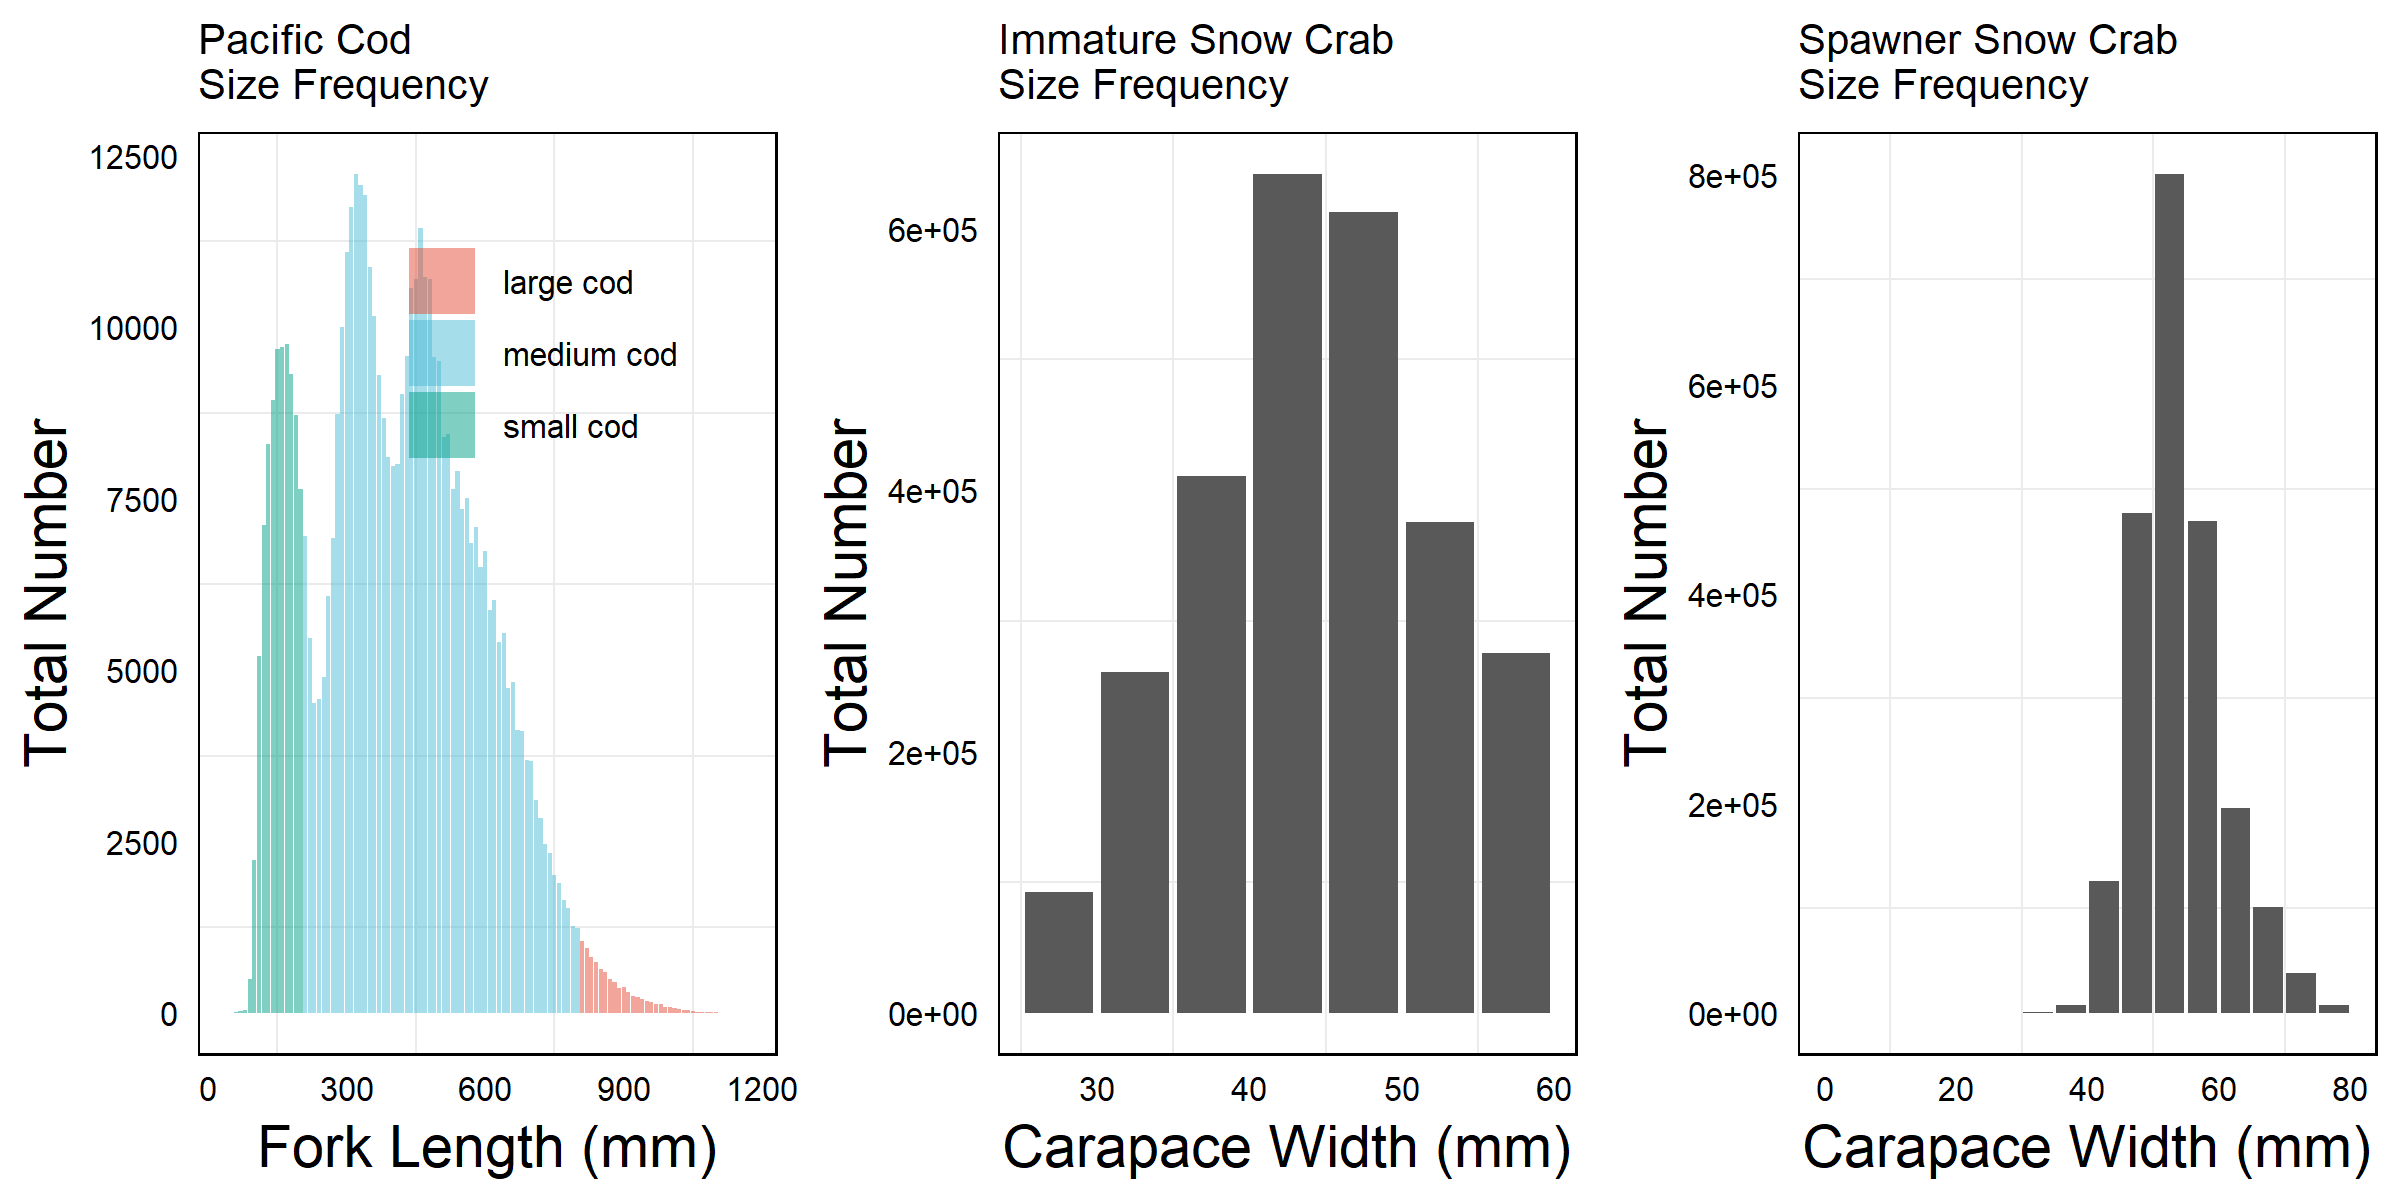
\includegraphics[width=33.33in]{C:/Users/Owen.Liu/Documents/github/cod_vs_crab/manuscript/figures/size_freq_all} \caption{Size-frequency distributions for the five classes included in the model, including all observations (n=103,550 observations)}\label{fig:sfreq}
\end{figure}

\hypertarget{maps-of-spatial-and-spatio-temporal-factors}{%
\subsection{Maps of spatial and spatio-temporal factors}\label{maps-of-spatial-and-spatio-temporal-factors}}

\begin{figure}
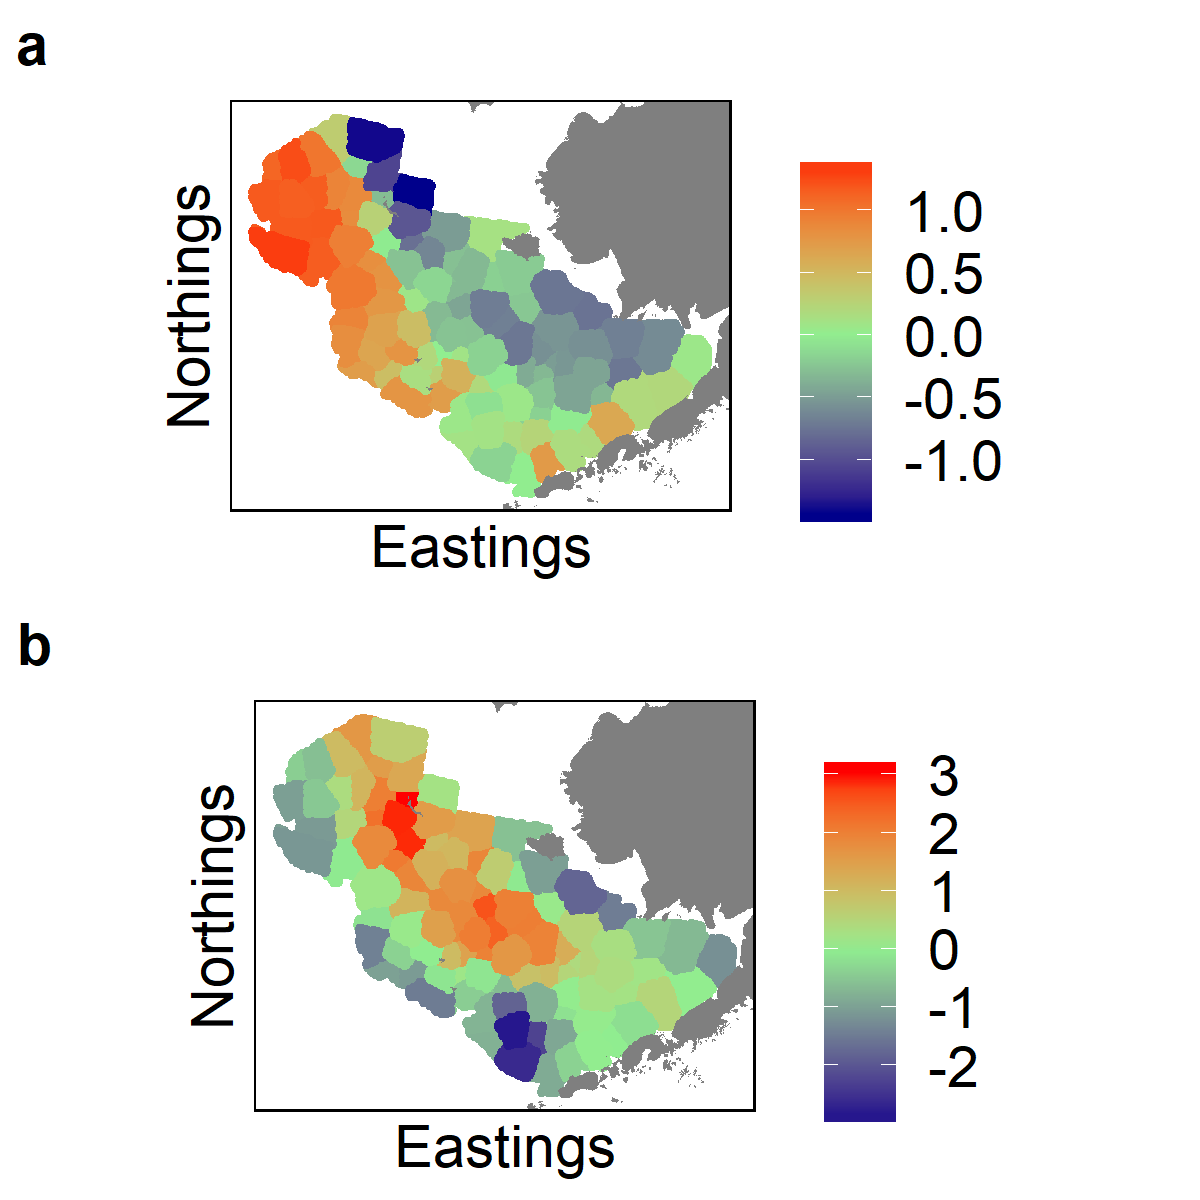
\includegraphics[width=16.67in]{C:/Users/Owen.Liu/Documents/github/cod_vs_crab/manuscript/figures/omega3s} \caption{The third spatial factor for average encounter rate (a) and positive abundance (b). Warmer colors represent positive values of the factor, while cool colors represent negative values.}\label{fig:omega13}
\end{figure}

\begin{figure}
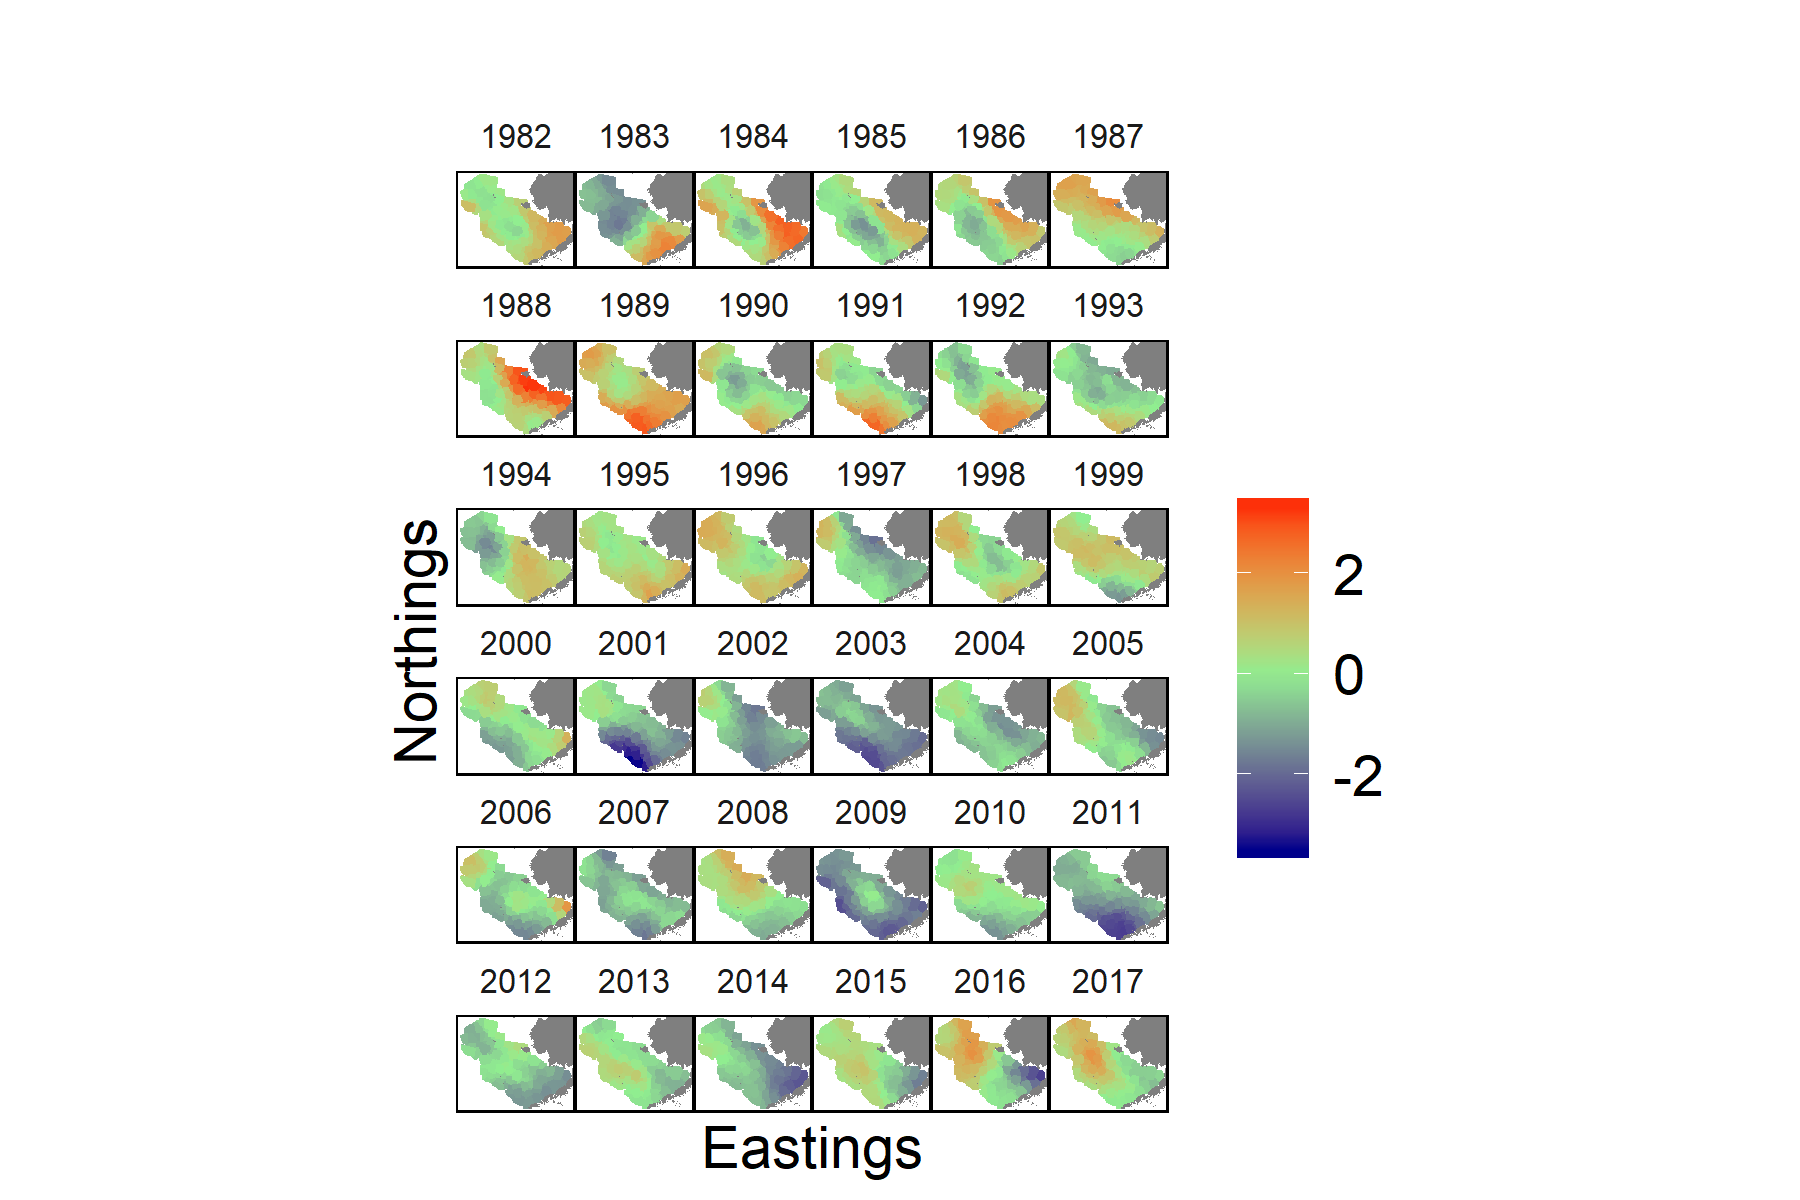
\includegraphics[width=25in]{C:/Users/Owen.Liu/Documents/github/cod_vs_crab/manuscript/figures/epsilon12} \caption{Values of the second spatio-temporal factor for encounter probability in each year in the study. Warmer colors represent positive values of the factor, while cooler colors represent negative values.}\label{fig:epsilon12}
\end{figure}

\begin{figure}
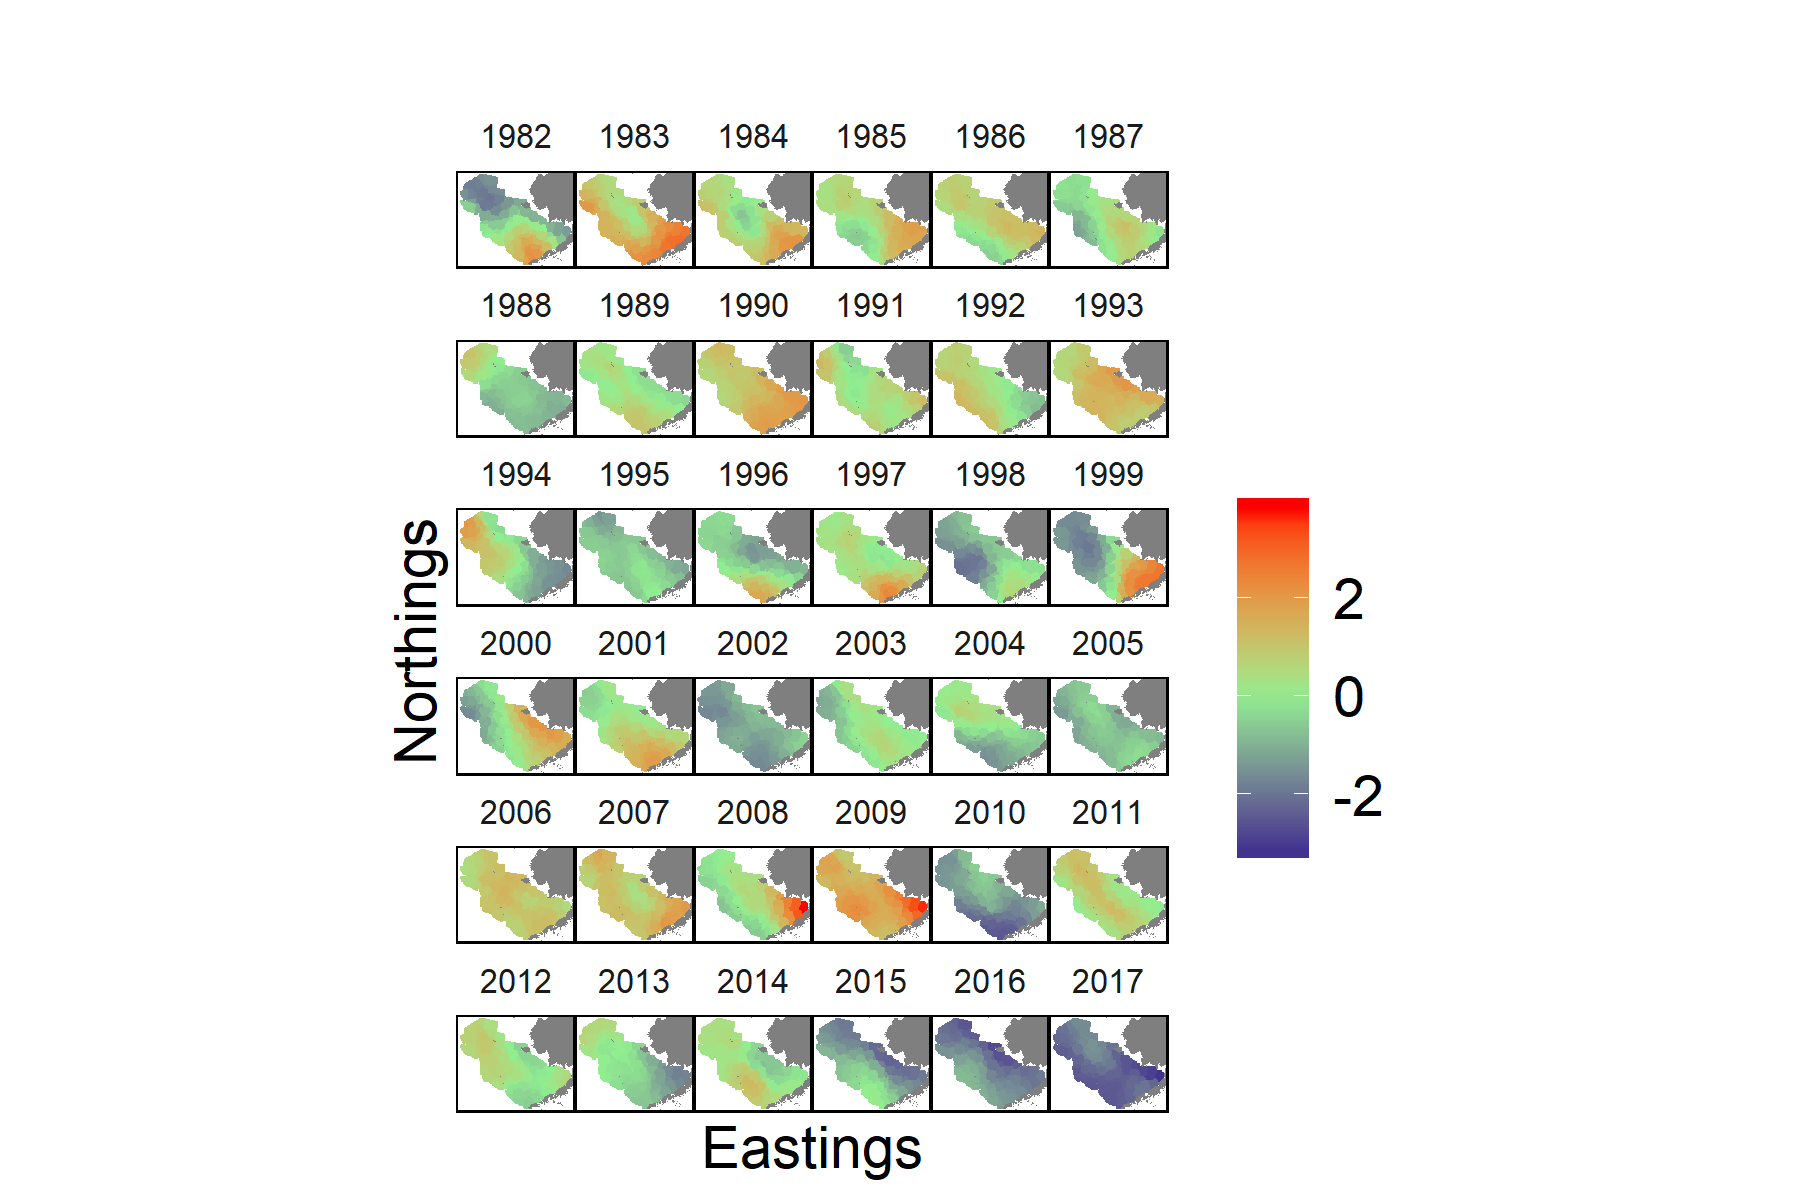
\includegraphics[width=25in]{C:/Users/Owen.Liu/Documents/github/cod_vs_crab/manuscript/figures/epsilon13} \caption{Values of the third spatio-temporal factor for encounter probability in each year in the study. Warmer colors represent positive values of the factor, while cooler colors represent negative values.}\label{fig:epsilon13}
\end{figure}

\begin{figure}
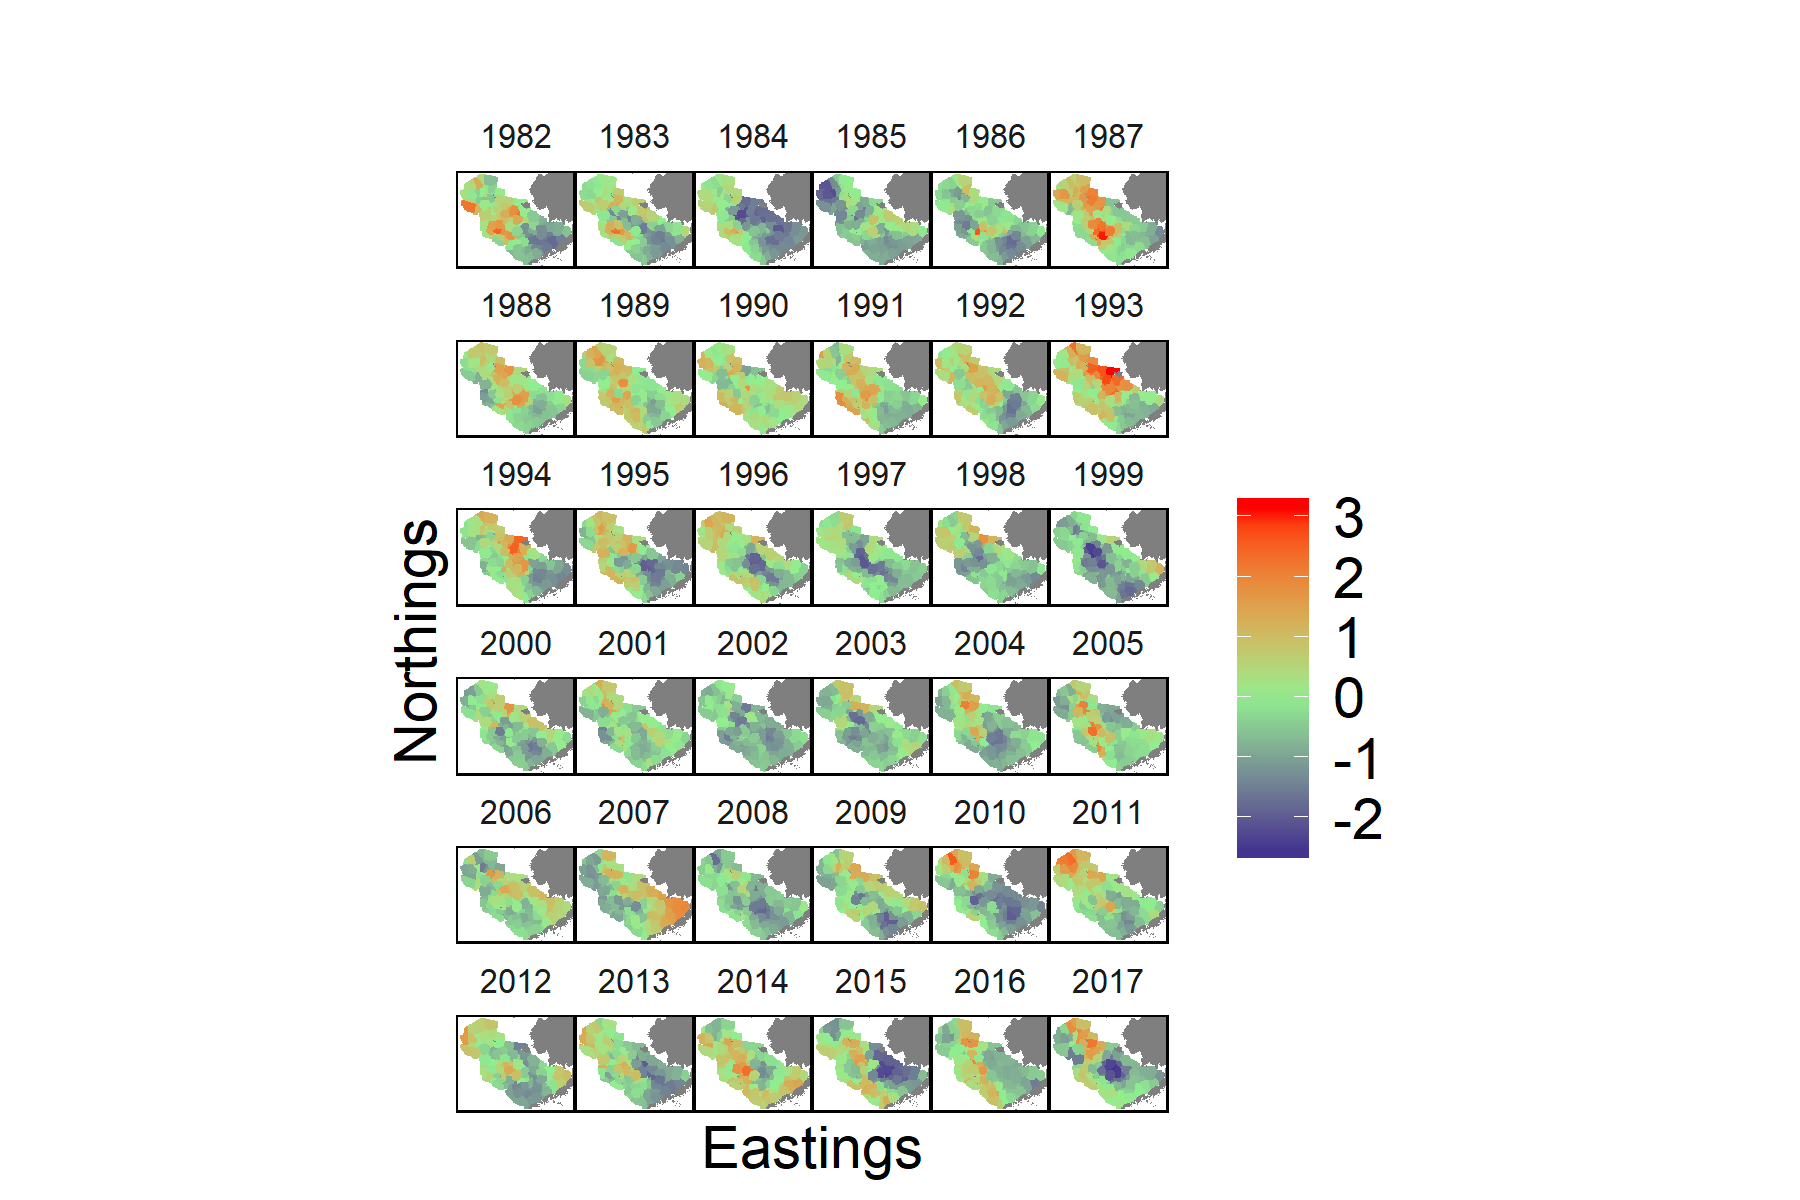
\includegraphics[width=25in]{C:/Users/Owen.Liu/Documents/github/cod_vs_crab/manuscript/figures/epsilon21} \caption{Values of the first spatio-temporal factor for positive abundance in each year in the study. Warmer colors represent positive values of the factor, while cooler colors represent negative values.}\label{fig:epsilon21}
\end{figure}

\begin{figure}
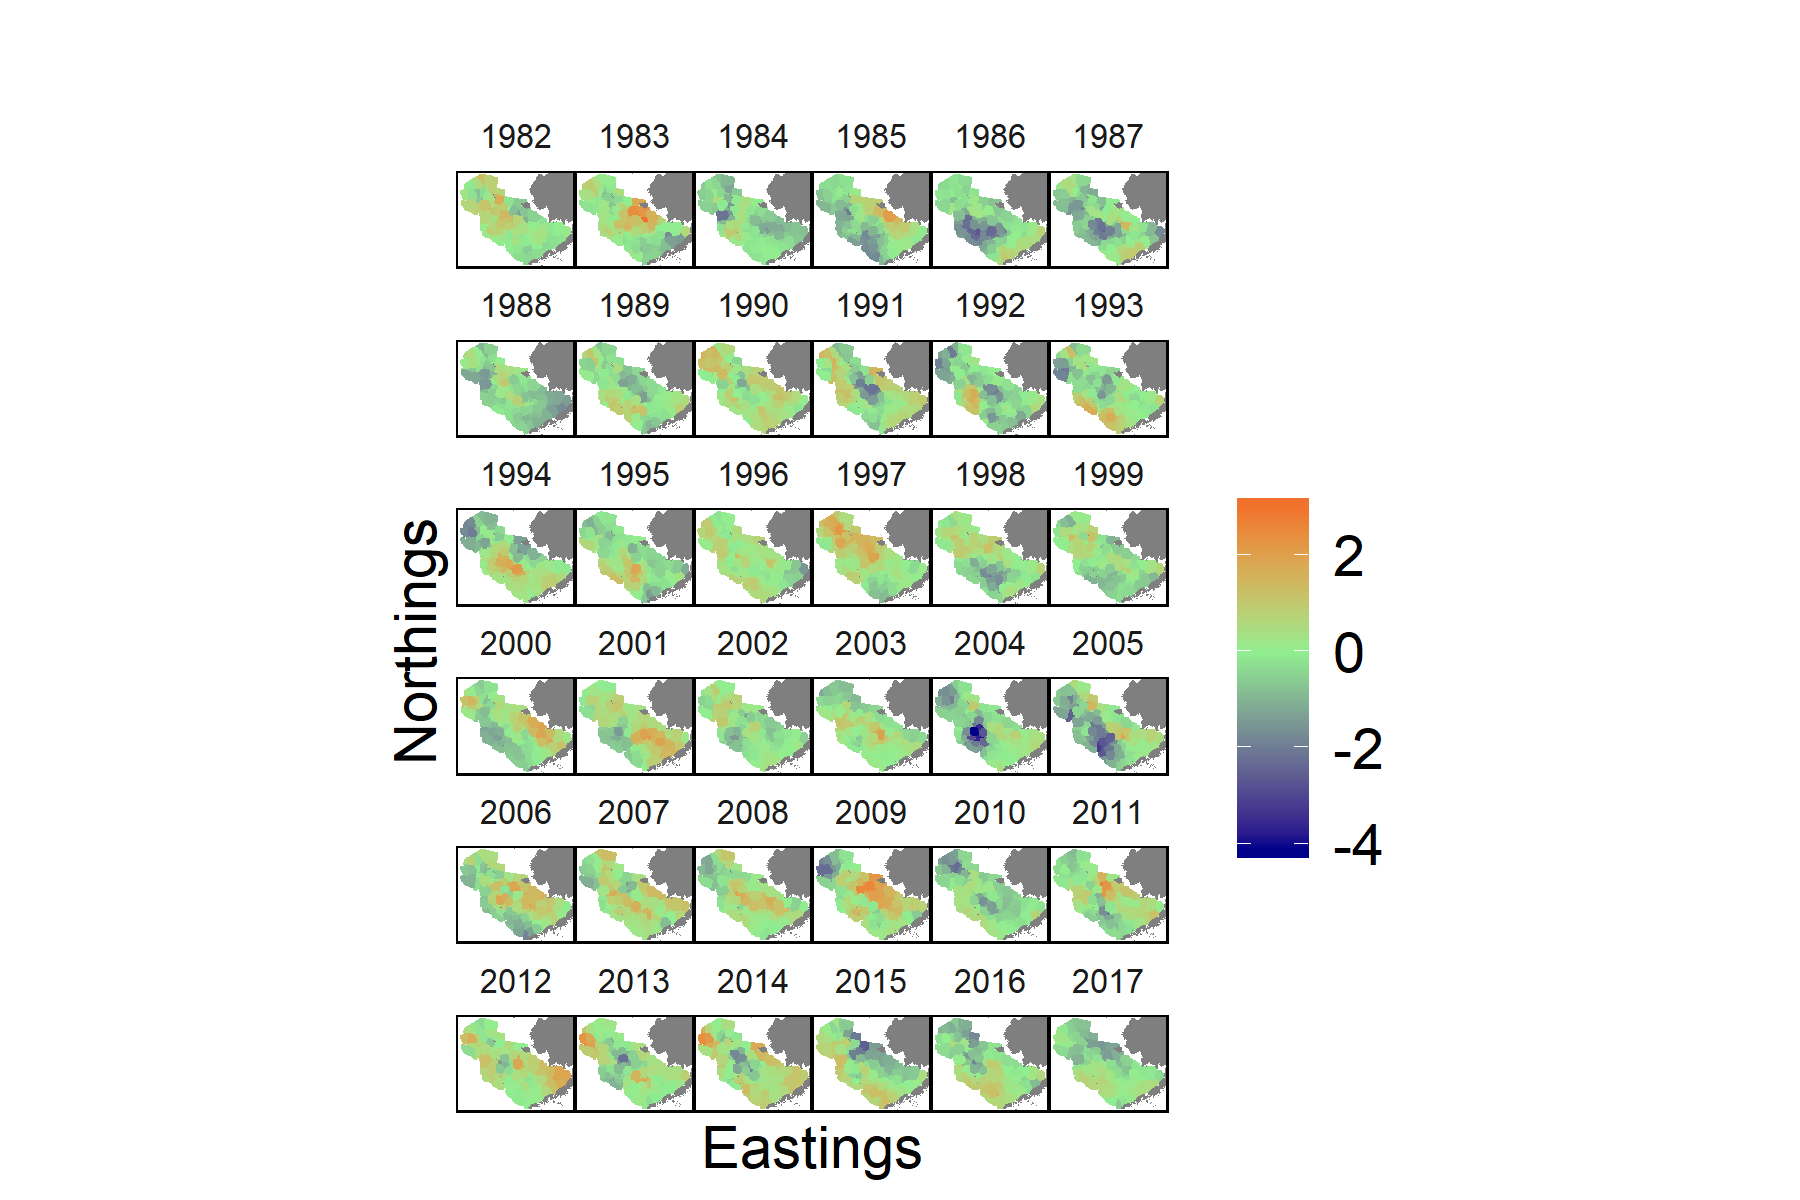
\includegraphics[width=25in]{C:/Users/Owen.Liu/Documents/github/cod_vs_crab/manuscript/figures/epsilon22} \caption{Values of the second spatio-temporal factor for encounter probability in each year in the study. Warmer colors represent positive values of the factor, while cooler colors represent negative values.}\label{fig:epsilon22}
\end{figure}

\begin{figure}
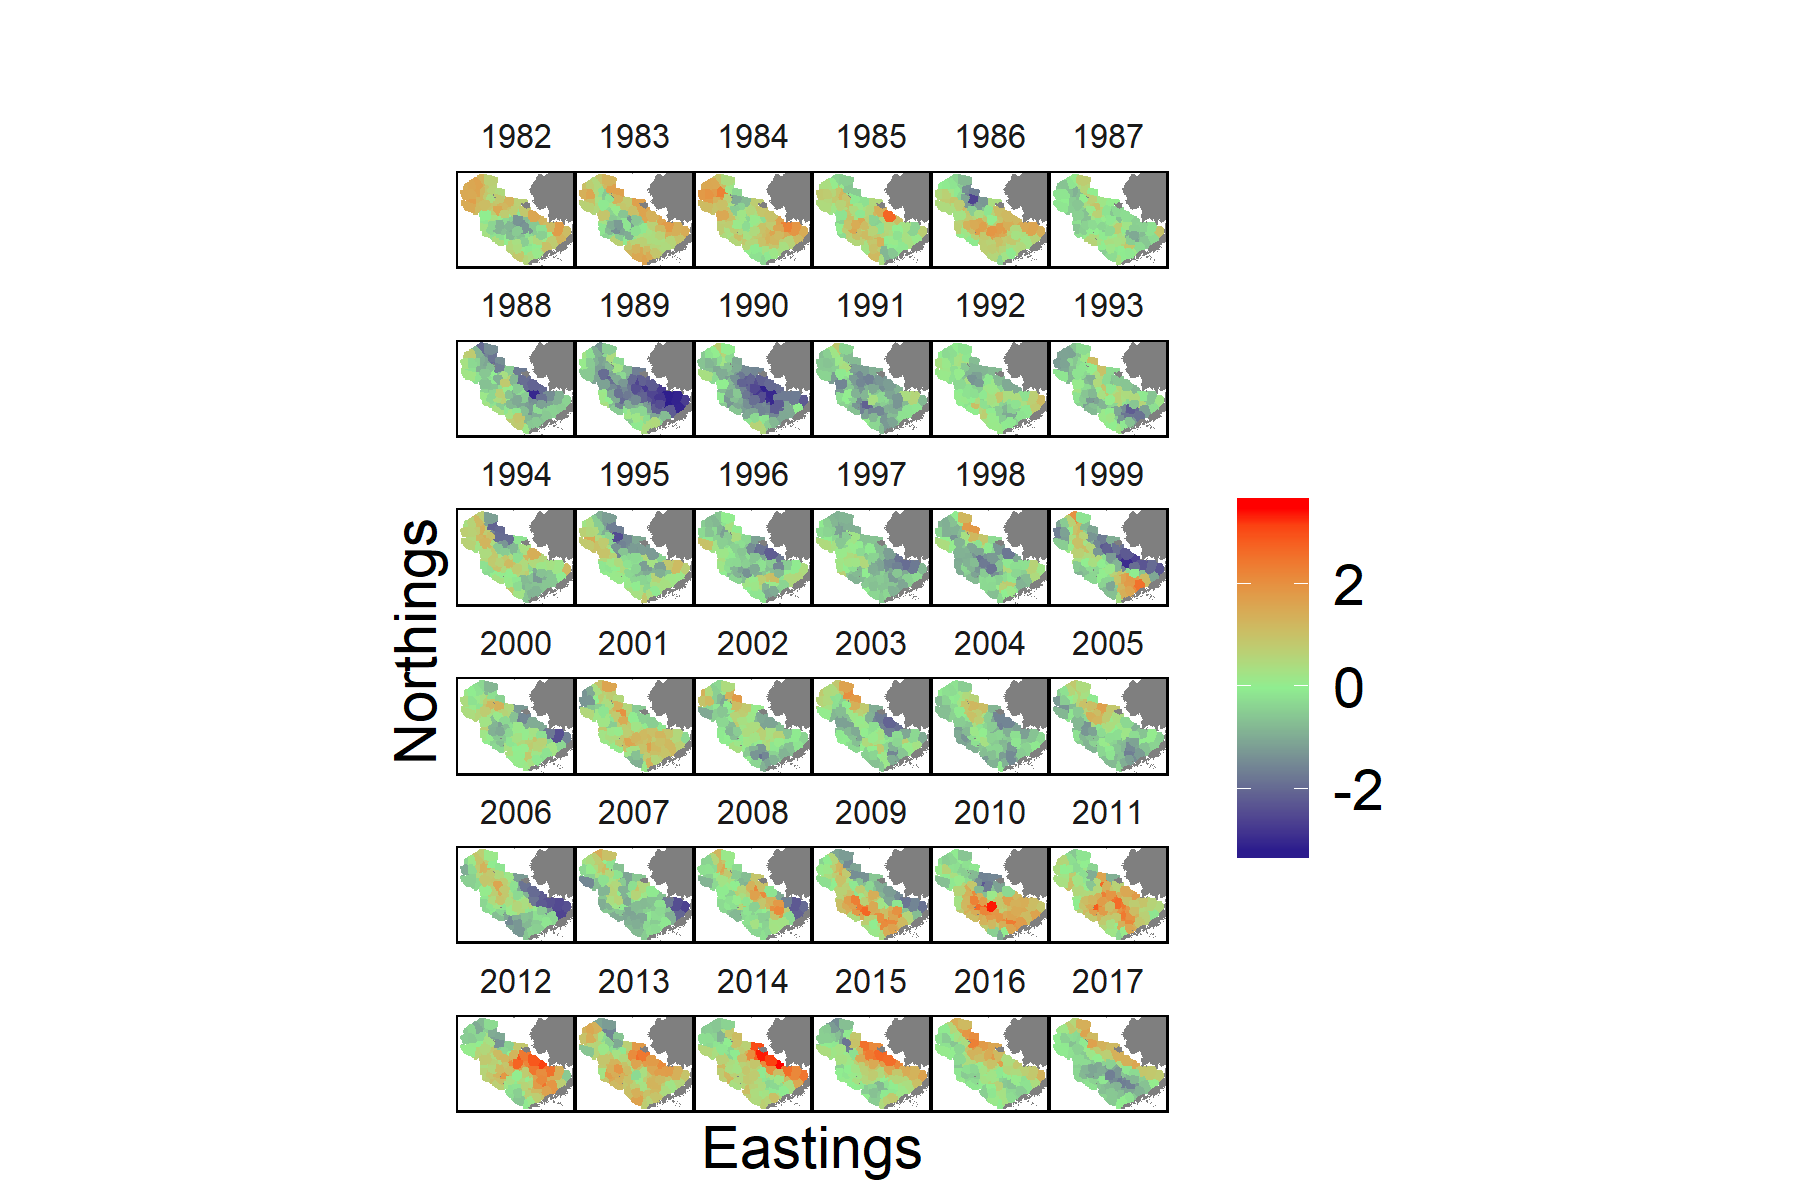
\includegraphics[width=25in]{C:/Users/Owen.Liu/Documents/github/cod_vs_crab/manuscript/figures/epsilon23} \caption{Values of the third spatio-temporal factor for encounter probability in each year in the study. Warmer colors represent positive values of the factor, while cooler colors represent negative values.}\label{fig:epsilon23}
\end{figure}

\hypertarget{predicted-density}{%
\subsection{Predicted density}\label{predicted-density}}

\begin{figure}
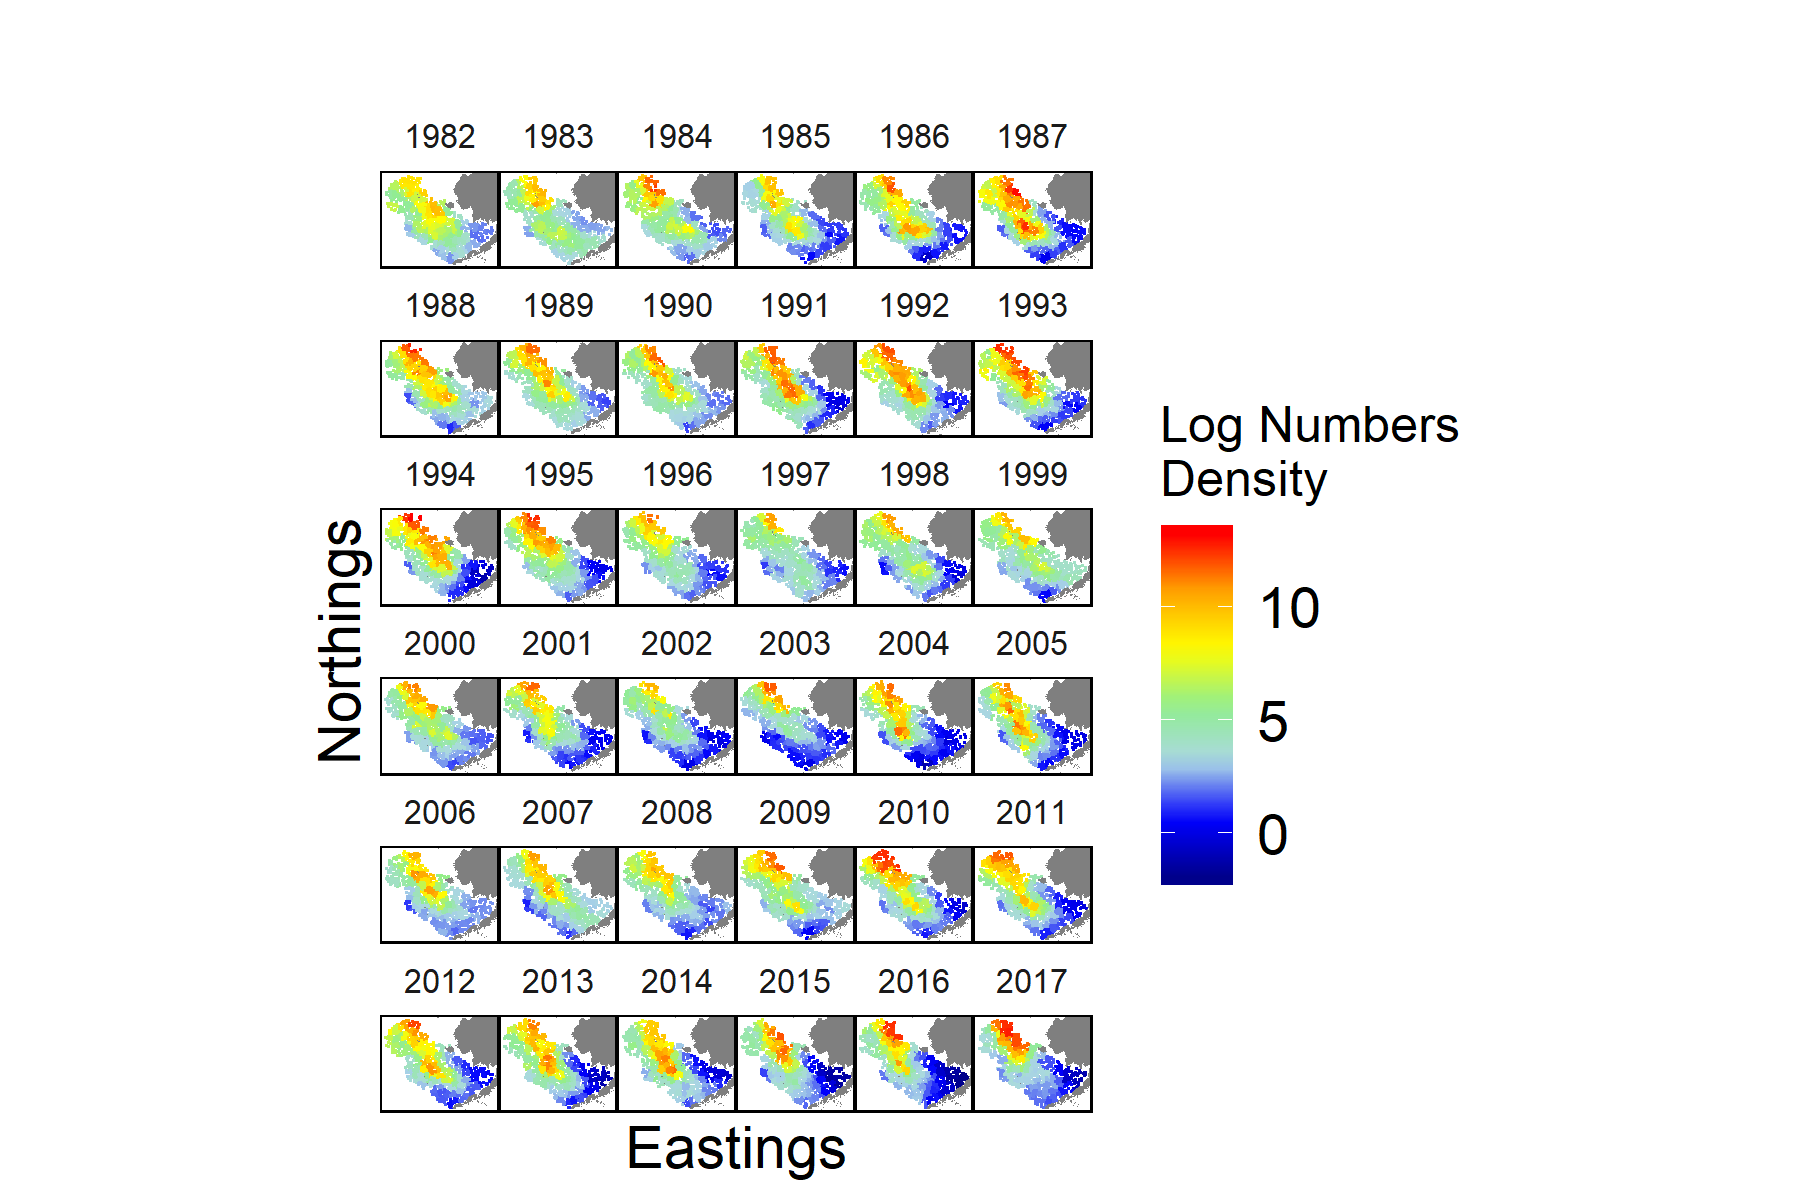
\includegraphics[width=25in]{C:/Users/Owen.Liu/Documents/github/cod_vs_crab/manuscript/figures/crab_abun} \caption{Predicted log-abundance of immature snow crab across the EBS in each year in the study}\label{fig:crabdens}
\end{figure}

\begin{figure}
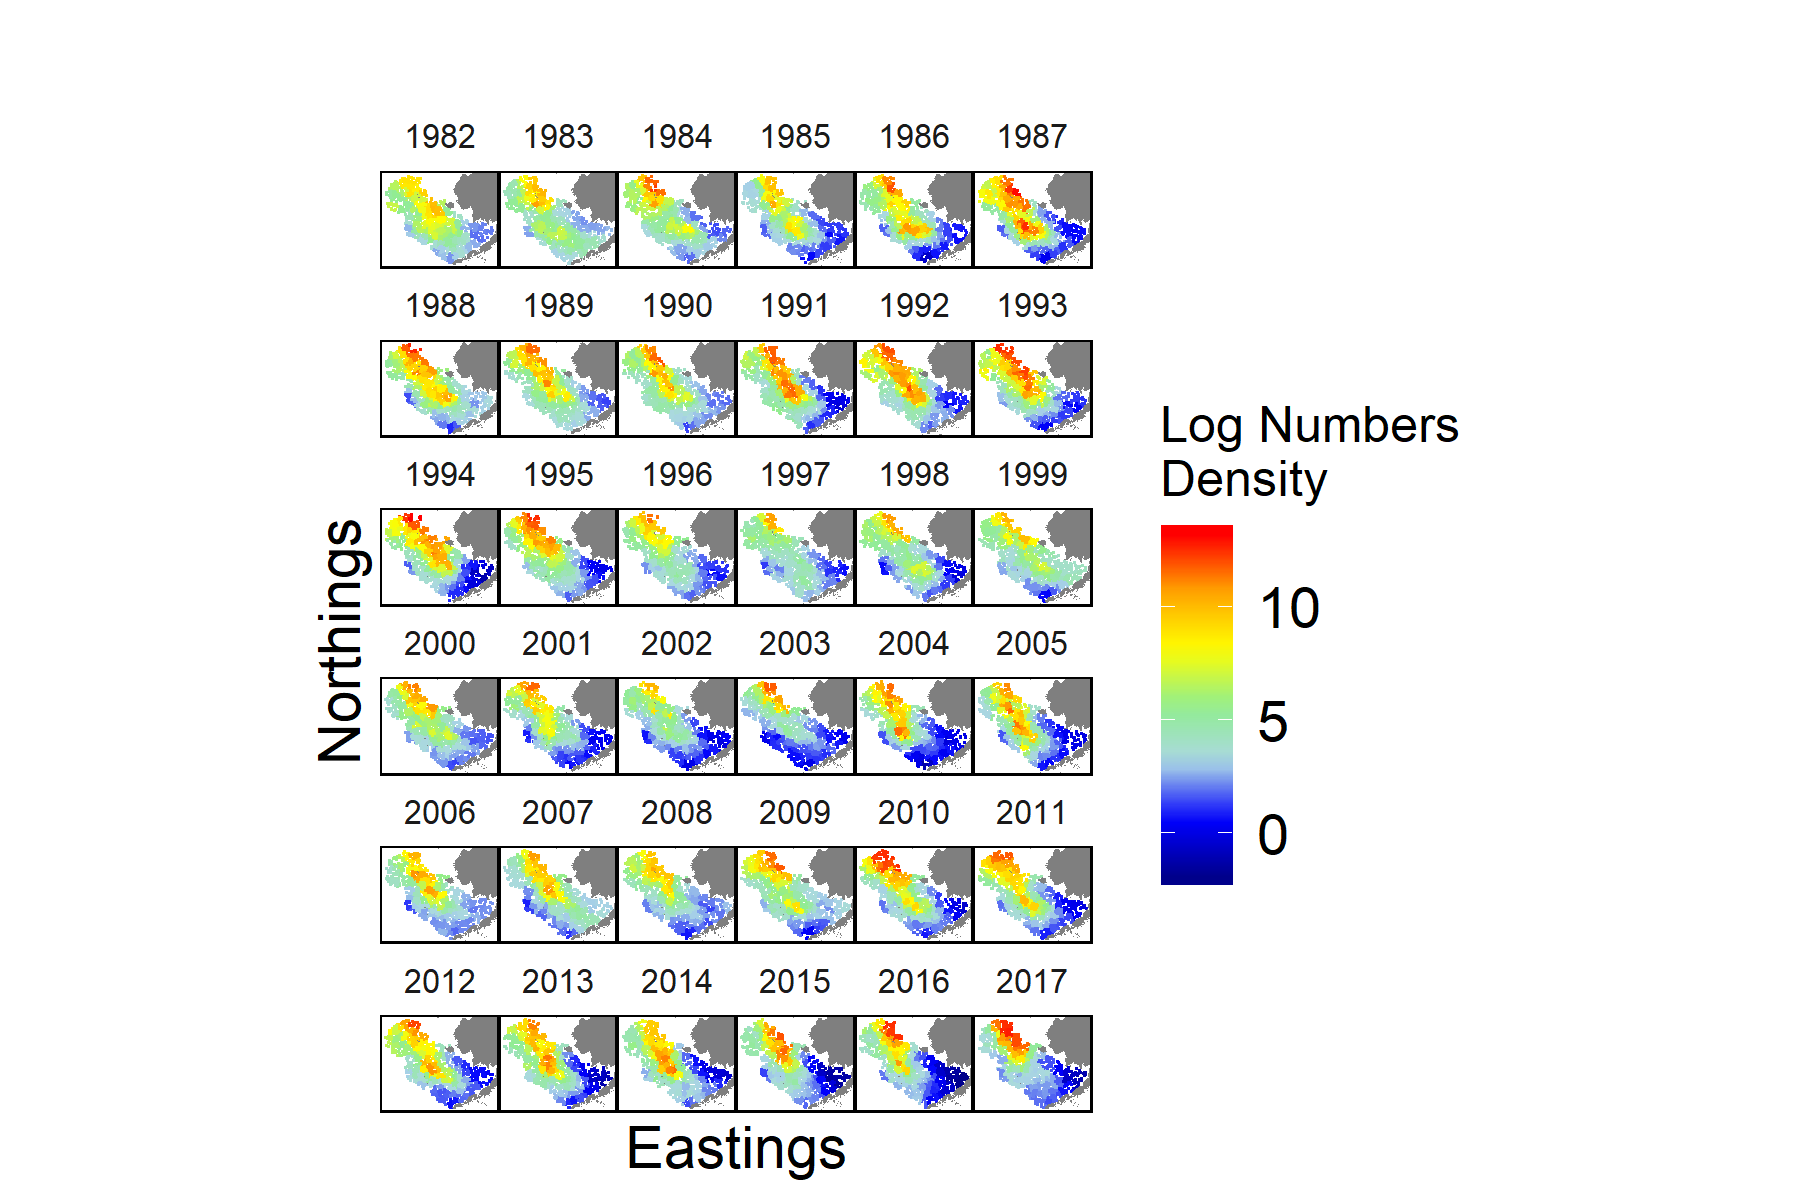
\includegraphics[width=25in]{C:/Users/Owen.Liu/Documents/github/cod_vs_crab/manuscript/figures/med_cod_abun} \caption{Predicted log-abundance of medium-sized Pacific cod across the EBS in each year in the study}\label{fig:coddens}
\end{figure}

\hypertarget{references}{%
\section*{References}\label{references}}
\addcontentsline{toc}{section}{References}

\hypertarget{refs}{}
\leavevmode\hypertarget{ref-Pikitch2004}{}%
1. Pikitch, E. K. \emph{et al.} Ecosystem-Based Fishery Management. \emph{Science} \textbf{300,} 2003--2003 (2004).

\leavevmode\hypertarget{ref-Fogarty2014}{}%
2. Fogarty, M. The art of ecosystem-based fishery management. \emph{Canadian Journal of Fisheries and Aquatic Sciences} \textbf{71,} 479--490 (2014).

\leavevmode\hypertarget{ref-Pitcher2009}{}%
3. Pitcher, T. J., Kalikoski, D., Short, K., Varkey, D. \& Pramod, G. An evaluation of progress in implementing ecosystem-based management of fisheries in 33 countries. \emph{Marine Policy} \textbf{33,} 223--232 (2009).

\leavevmode\hypertarget{ref-Orio2019}{}%
4. Orio, A. \emph{et al.} Spatial contraction of demersal fish populations in a large marine ecosystem. \emph{Journal of Biogeography} 633--645 (2019). doi:\href{https://doi.org/10.1111/jbi.13510}{10.1111/jbi.13510}

\leavevmode\hypertarget{ref-Hollowed2000}{}%
5. Hollowed, A. B. \emph{et al.} Are multispecies models an improvement on single-species models for measuring fishing impacts on marine ecosystems? \emph{ICES Journal of Marine Science: Journal du Conseil} \textbf{57,} 707--719 (2000).

\leavevmode\hypertarget{ref-Swain2012}{}%
6. Swain, D. P. \& Mohn, R. K. Forage fish and the factors governing recovery of Atlantic cod ( Gadus morhua ) on the eastern Scotian Shelf. \emph{Canadian Journal of Fisheries and Aquatic Sciences} \textbf{69,} 997--1001 (2012).

\leavevmode\hypertarget{ref-Hollowed2000a}{}%
7. Hollowed, A. B., Ianelli, J. N. \& Livingston, P. a. Including predation mortality in stock assessments: a case study for Gulf of Alaska walleye pollock. \emph{ICES Journal of Marine Science} \textbf{57,} 279--293 (2000).

\leavevmode\hypertarget{ref-Pagel2012}{}%
8. Pagel, J. \& Schurr, F. M. Forecasting species ranges by statistical estimation of ecological niches and spatial population dynamics. \emph{Global Ecology and Biogeography} \textbf{21,} 293--304 (2012).

\leavevmode\hypertarget{ref-Szuwalski2015}{}%
9. Szuwalski, C. S., Vert-Pre, K. A., Punt, A. E., Branch, T. A. \& Hilborn, R. Examining common assumptions about recruitment: A meta-analysis of recruitment dynamics for worldwide marine fisheries. \emph{Fish and Fisheries} \textbf{16,} 633--648 (2015).

\leavevmode\hypertarget{ref-Kempf2010}{}%
10. Kempf, A., Huse, G., Dingsør, G., Floeter, J. \& Temming, A. The importance of overlap -- predicting North Sea cod recovery with a multi species fisheries assessment model. \emph{ICES Journal of Marine Science} \textbf{67,} 1989--1997 (2010).

\leavevmode\hypertarget{ref-Frank2016}{}%
11. Frank, K. T., Petrie, B., Leggett, W. C. \& Boyce, D. G. Large scale, synchronous variability of marine fish populations driven by commercial exploitation. \emph{Proceedings of the National Academy of Sciences} \textbf{113,} 8248--8253 (2016).

\leavevmode\hypertarget{ref-Swain2019}{}%
12. Swain, D. P., Benoît, H. P., Hammill, M. O. \& Sulikowski, J. A. Risk of extinction of a unique skate population due to predation by a recovering marine mammal. \emph{Ecological Applications} e01921 (2019). doi:\href{https://doi.org/10.1002/eap.1921}{10.1002/eap.1921}

\leavevmode\hypertarget{ref-Parada2010}{}%
13. Parada, C., Armstrong, D. A., Ernst, B., Hinckley, S. \& Orensanz, J. M. Spatial dynamics of snow crab (chionoecetes opilio) in the eastern bering sea-putting together the pieces of the puzzle. \emph{Bulletin of Marine Science} \textbf{86,} 413--437 (2010).

\leavevmode\hypertarget{ref-NPFMC2018}{}%
14. Szuwalski, C. \emph{A stock assessment for eastern Bering Sea snow crab}. 1--89 (North Pacific Fishery Management Council, 2018).

\leavevmode\hypertarget{ref-Zheng2006}{}%
15. Zheng, J. \& Kruse, G. H. Recruitment variation of eastern Bering Sea crabs: Climate-forcing or top-down effects? \emph{Progress in Oceanography} \textbf{68,} 184--204 (2006).

\leavevmode\hypertarget{ref-Orensanz2004}{}%
16. Orensanz, J. L., Ernst, B., Armstrong, D. A., Stabeno, P. J. \& Livingston, P. Contraction of the geographic range of distribution of snow crab (Chionoecetes Opilio) in the Eastern Bering Sea : an environmental ratchet ? \emph{CalCOFI Reports} \textbf{45,} 65--79 (2004).

\leavevmode\hypertarget{ref-Wyllie-Echeverria1998}{}%
17. Wyllie-Echeverria, T. \& Wooster, W. S. Year-to-year variations in Bering Sea ice cover and some consequences for fish distributions. \emph{Fisheries Oceanography} \textbf{7,} 159--170 (1998).

\leavevmode\hypertarget{ref-Ernst2005}{}%
18. Ernst, B., Orensanz, J. (. \& Armstrong, D. A. Spatial dynamics of female snow crab (Chionoecetes opilio) in the eastern Bering Sea. \emph{Canadian Journal of Fisheries and Aquatic Sciences} \textbf{62,} 2673 (2005).

\leavevmode\hypertarget{ref-Ernst2012}{}%
19. Ernst, B., Armstrong, D. A., Burgos, J. \& Orensanz, J. (. Life history schedule and periodic recruitment of female snow crab (Chionoecetes opilio) in the eastern Bering Sea. \emph{Canadian Journal of Fisheries and Aquatic Sciences} \textbf{69,} 532--550 (2012).

\leavevmode\hypertarget{ref-Livingston1989}{}%
20. Livingston, P. A. Interannual trends in Pacific cod, Gadus macrocephalus, predation on three commercially important crab species in the eastern Bering Sea. \emph{Fishery Bulletin} \textbf{87,} 807--827 (1989).

\leavevmode\hypertarget{ref-Burgos2013}{}%
21. Burgos, J., Ernst, B., Armstrong, D. \& Orensanz, J. M. Fluctuations in range and abundance of snow crab (Chionoecetes opilio) from the eastern bering sea: What role for pacific cod (Gadus macrocephalus) predation? \emph{Bulletin of Marine Science} \textbf{89,} 57--81 (2013).

\leavevmode\hypertarget{ref-Chabot2008}{}%
22. Chabot, D., Sainte-Marie, B., Briand, K. \& Hanson, J. M. Atlantic cod and snow crab predator-prey size relationship in the Gulf of St. Lawrence, Canada. \emph{Marine Ecology Progress Series} \textbf{363,} 227--240 (2008).

\leavevmode\hypertarget{ref-Hurst2012}{}%
23. Hurst, T. P., Moss, J. H. \& Miller, J. A. Distributional patterns of 0-group Pacific cod (Gadus macrocephalus) in the eastern Bering SEas under variable recruitment and thermal conditions. \emph{ICES Journal of Marine Science} \textbf{69,} 163--174 (2012).

\leavevmode\hypertarget{ref-Thorson2016}{}%
24. Thorson, J. T. \emph{et al.} Joint dynamic species distribution models: a tool for community ordination and spatio-temporal monitoring. \emph{Global Ecology and Biogeography} (2016). doi:\href{https://doi.org/10.1111/geb.12464}{10.1111/geb.12464}

\leavevmode\hypertarget{ref-Thorson2019}{}%
25. Thorson, J. T. Guidance for decisions using the Vector Autoregressive Spatio-Temporal (VAST) package in stock, ecosystem, habitat and climate assessments. \emph{Fisheries Research} \textbf{210,} 143--161 (2019).

\leavevmode\hypertarget{ref-Lindgren2011}{}%
26. Lindgren, F., Rue, H. \& Lindstrom, J. An explicit link between Gaussian fields and Gaussian Markov random fields: the stochastic partial differential equation approach. \emph{Journal of the Royal Statistical Society. Series B} \textbf{73,} 423--498 (2011).

\leavevmode\hypertarget{ref-Illian2012}{}%
27. Illian, J. B., Sørbye, S. H. \& Rue, H. A toolbox for fitting complex spatial point process models using integrated nested Laplace approximation (INLA). \emph{Annals of Applied Statistics} \textbf{6,} 1499--1530 (2012).

\leavevmode\hypertarget{ref-Kristensen2015}{}%
28. Kristensen, K., Nielsen, A., Berg, C. W., Skaug, H. \& Bell, B. TMB: Automatic Differentiation and Laplace Approximation. (2015). doi:\href{https://doi.org/10.18637/jss.v070.i05}{10.18637/jss.v070.i05}

\leavevmode\hypertarget{ref-Kotwicki2013}{}%
29. Kotwicki, S. \& Lauth, R. R. Detecting temporal trends and environmentally-driven changes in the spatial distribution of bottom fishes and crabs on the eastern Bering Sea shelf. \emph{Deep-Sea Research Part II: Topical Studies in Oceanography} \textbf{94,} 231--243 (2013).

\leavevmode\hypertarget{ref-Thompson2018}{}%
30. Thompson, G. G. \emph{Assessment of the Pacific Cod Stock in the Eastern Bering Sea}. 229--516 (North Pacific Fishery Management Council Stock Assessment; Fishery Evaluation, 2018).

\leavevmode\hypertarget{ref-Thorson2016a}{}%
31. Thorson, J. T., Pinsky, M. L. \& Ward, E. J. Model-based inference for estimating shifts in species distribution, area occupied and centre of gravity. \emph{Methods in Ecology and Evolution} \textbf{7,} 990--1002 (2016).


\end{document}
